%!TEX root = ../report.tex

\begin{document}
\chapter{Experimental Results}

\section{ Notes on Analysis }
TODO: add this section\?
note about common things like how Duckett Historical is actually live and future is using old data mapped to new
notes about cyclic and decay artifacts in accuracy over time

\section{ Doored Areas }

\subsection { Door A }

Given the periodic, human, and slightly random nature of Door A, it serves as
an excellent starting point and litmus test of for various spatio-temporal
world modeling techniques. Door A's results establish a trend that can be seen
throughout the rest of the results. This is particularly visible in figure 6.3
where the models accuracy are evaluated over time. \\

\begin{table}[h!]
  \centering
  \resizebox{\textwidth}{!}{%
    \begin{tabular}{|l|l|l|l|l|}
      \hline
      & Duckett & Gaussian & FreMEn  & HyperTime \\ \hline
      Historical Accuracy             & 84.11\% & 77.80\%  & 92.51\% & 97.66\%   \\ \hline
      Prediction Accuracy             & 77.15\% & 79.43\%  & 87.08\% & 88.87\%   \\ \hline
      Computation Time (Milliseconds) & 610     & 50       & 70      & 5630      \\ \hline
      Memory Usage (KB)               & 31036   & 34968    & 34656   & 37192     \\ \hline
    \end{tabular}%
  }
  \caption{Door A Data Overview}
\end{table}

Do to the periodic nature of the data, the techniques based off of extracting
periodicities (i.e. FreMEn and HyperTime) do an excellent job of recreating
passed events as well as predicting the future. HyperTime's slightly better
prediction is most likely due to the extra steps taken to wrap the data back
in on itself temporally.  This additional training and accuracy comes at a
great cost however. HyperTime manages only a small performance increase over
around one percent over FreMEn with a total training and prediction time
taking on the order of two magnitudes longer compared to either Gaussian or FreMEn.
Finally, it appears that the Gaussian model completely failed to predict any
open state.  This is thought to be due to the sparseness of positive, or open
states resulting in the model oscillating between 0 and just under 0.5 thus
never reaching the open threshold. \\

\begin{figure}
  \begin{tabular}{cc}
    {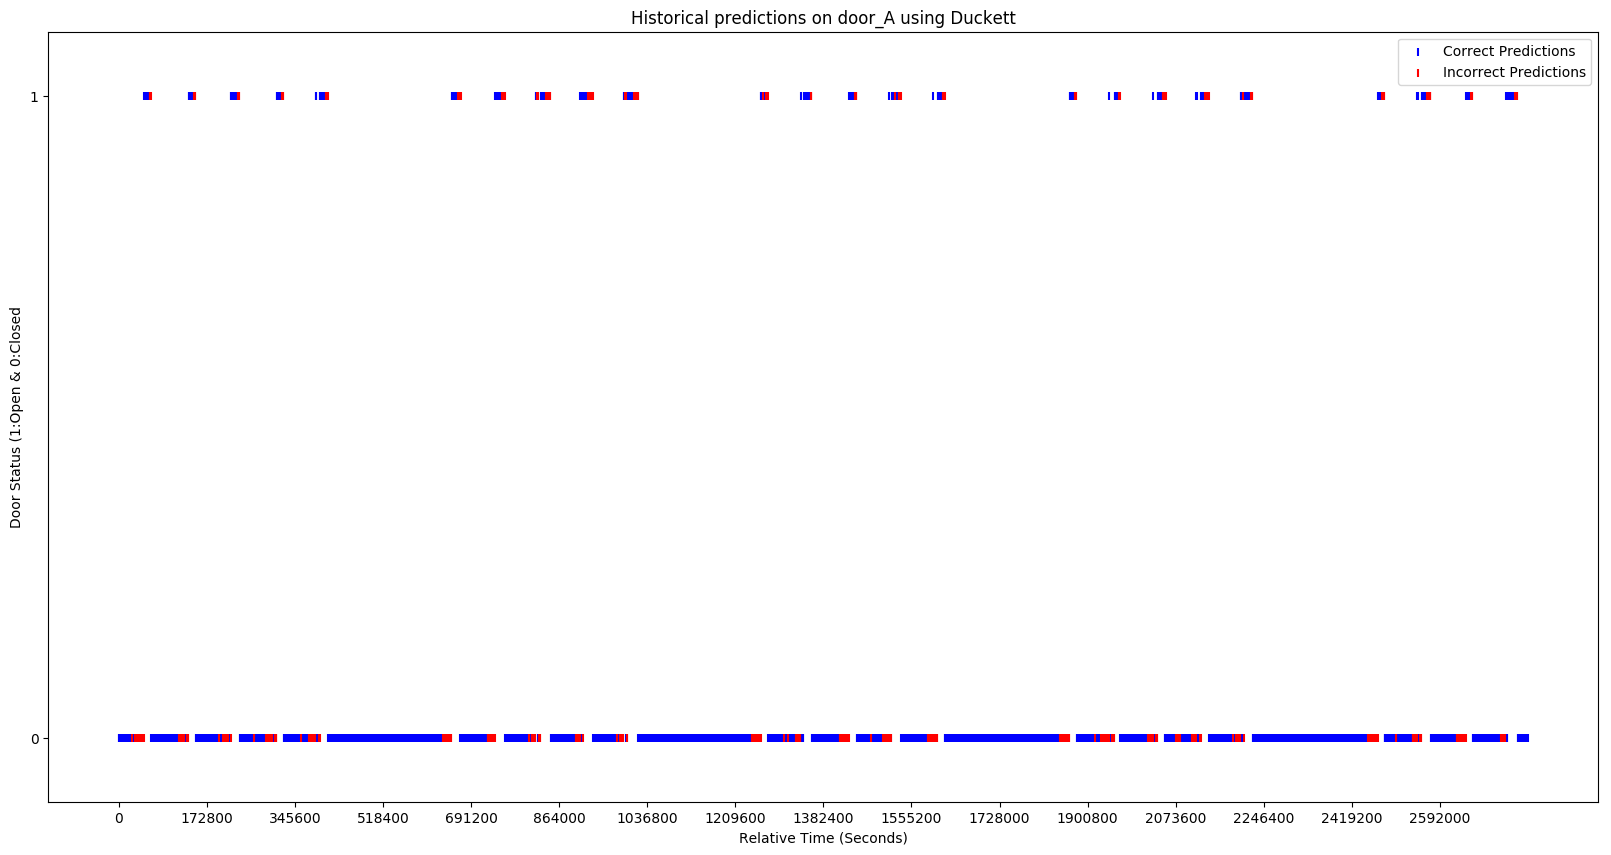
\includegraphics[width = 3in]{images/results/Historical_door_A_Duckett.png}} &
    {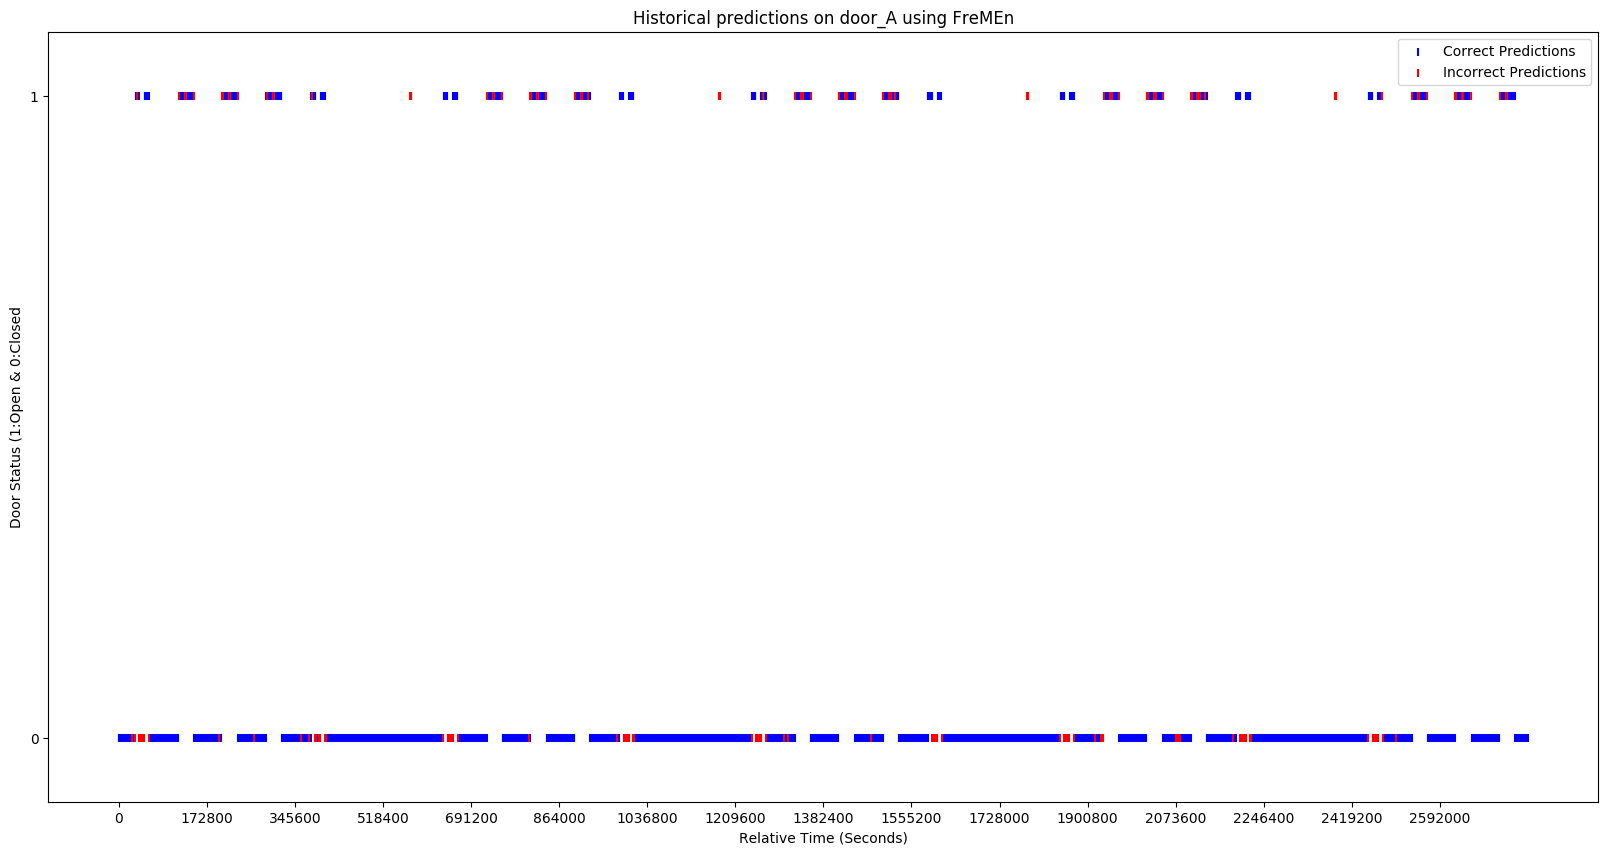
\includegraphics[width = 3in]{images/results/Historical_door_A_FreMEn.png}} \\
    {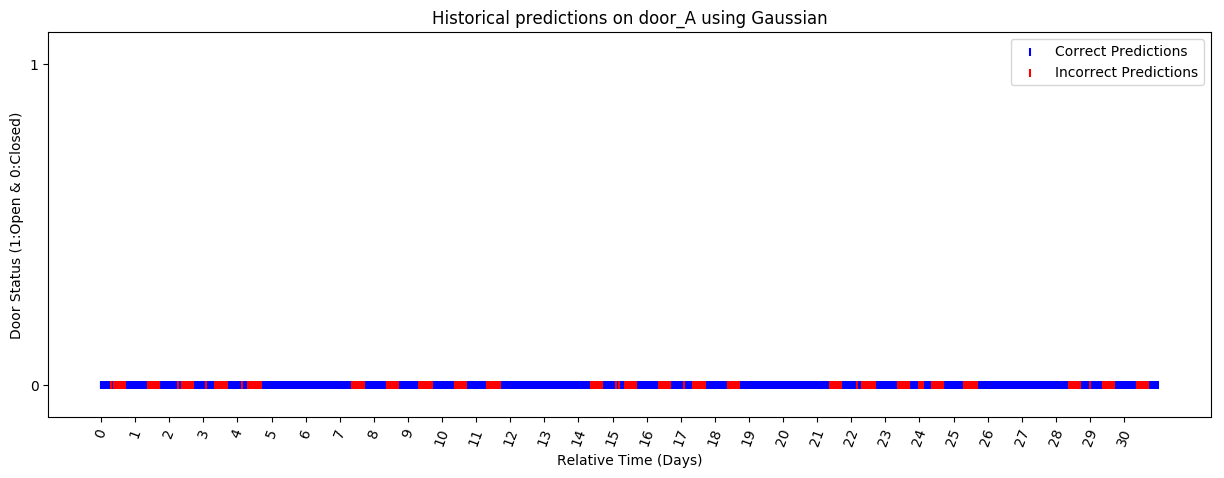
\includegraphics[width = 3in]{images/results/Historical_door_A_Gaussian.png}} &
    {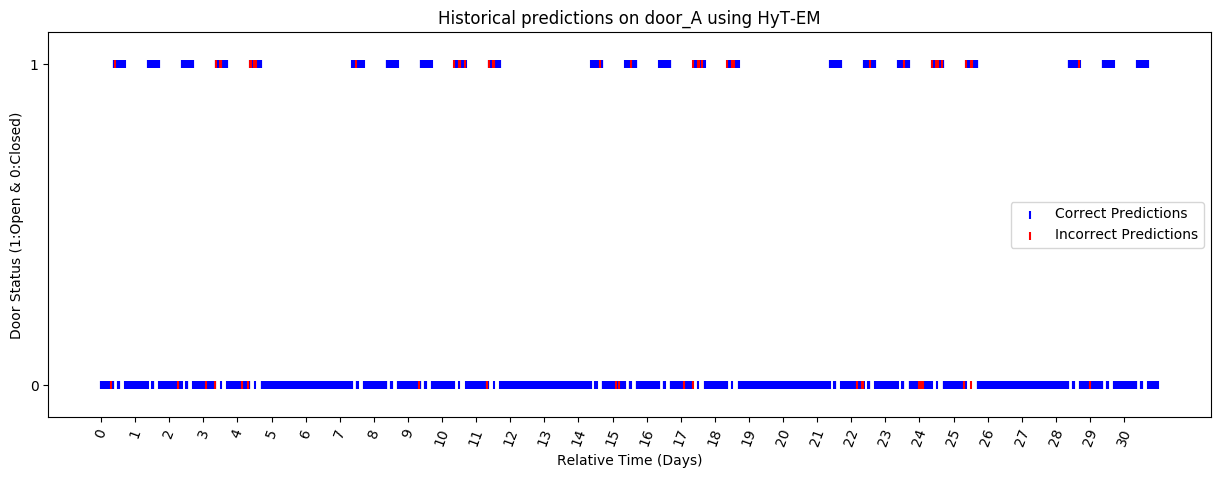
\includegraphics[width = 3in]{images/results/Historical_door_A_HyT-EM.png}} \\
  \end{tabular}
  \caption{Historical Recreations - Door A}
\end{figure} \\ \\

\begin{figure}
  \begin{tabular}{cc}
    {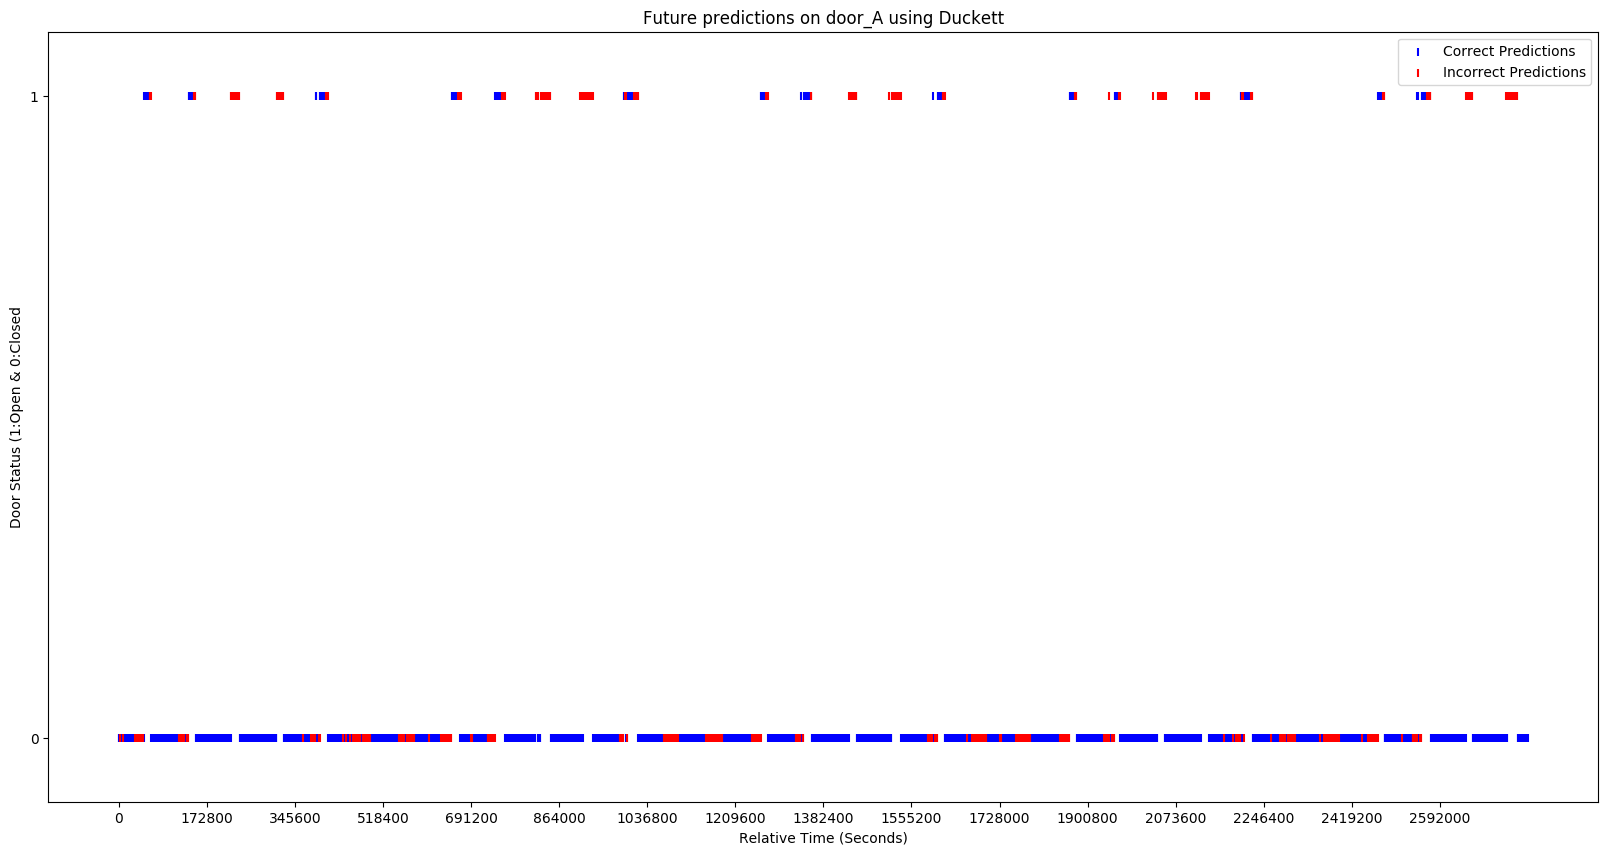
\includegraphics[width = 3in]{images/results/Future_door_A_Duckett.png}} &
    {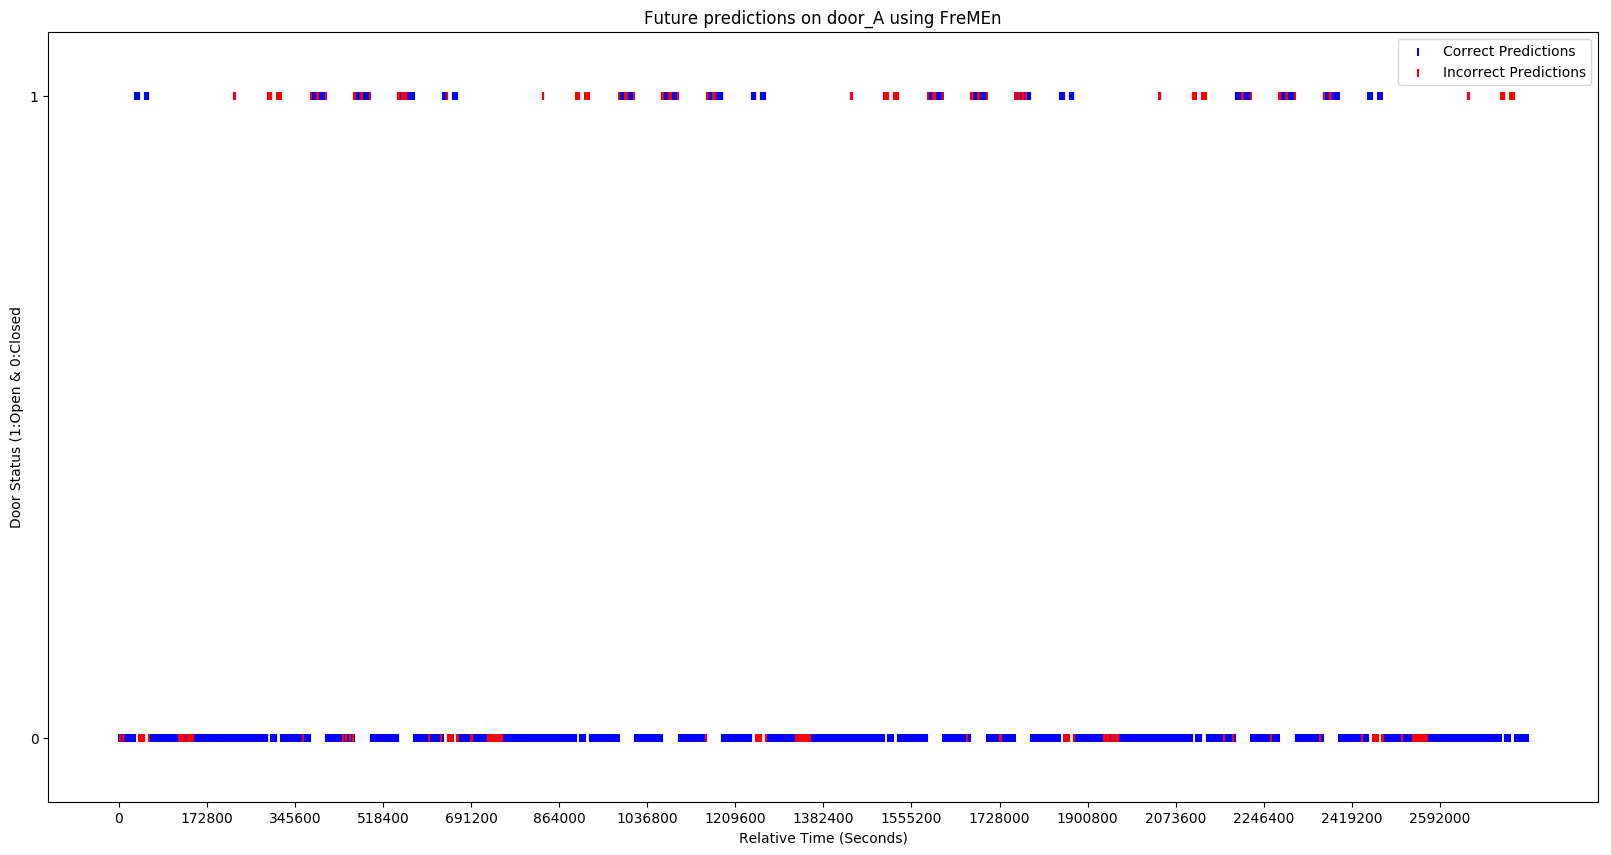
\includegraphics[width = 3in]{images/results/Future_door_A_FreMEn.png}} \\
    {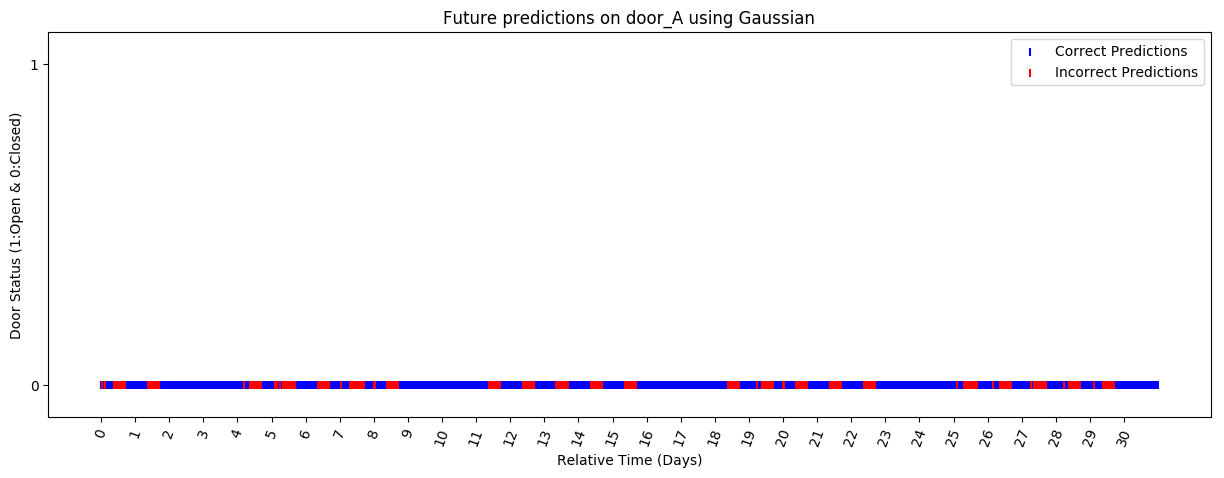
\includegraphics[width = 3in]{images/results/Future_door_A_Gaussian.png}} &
    {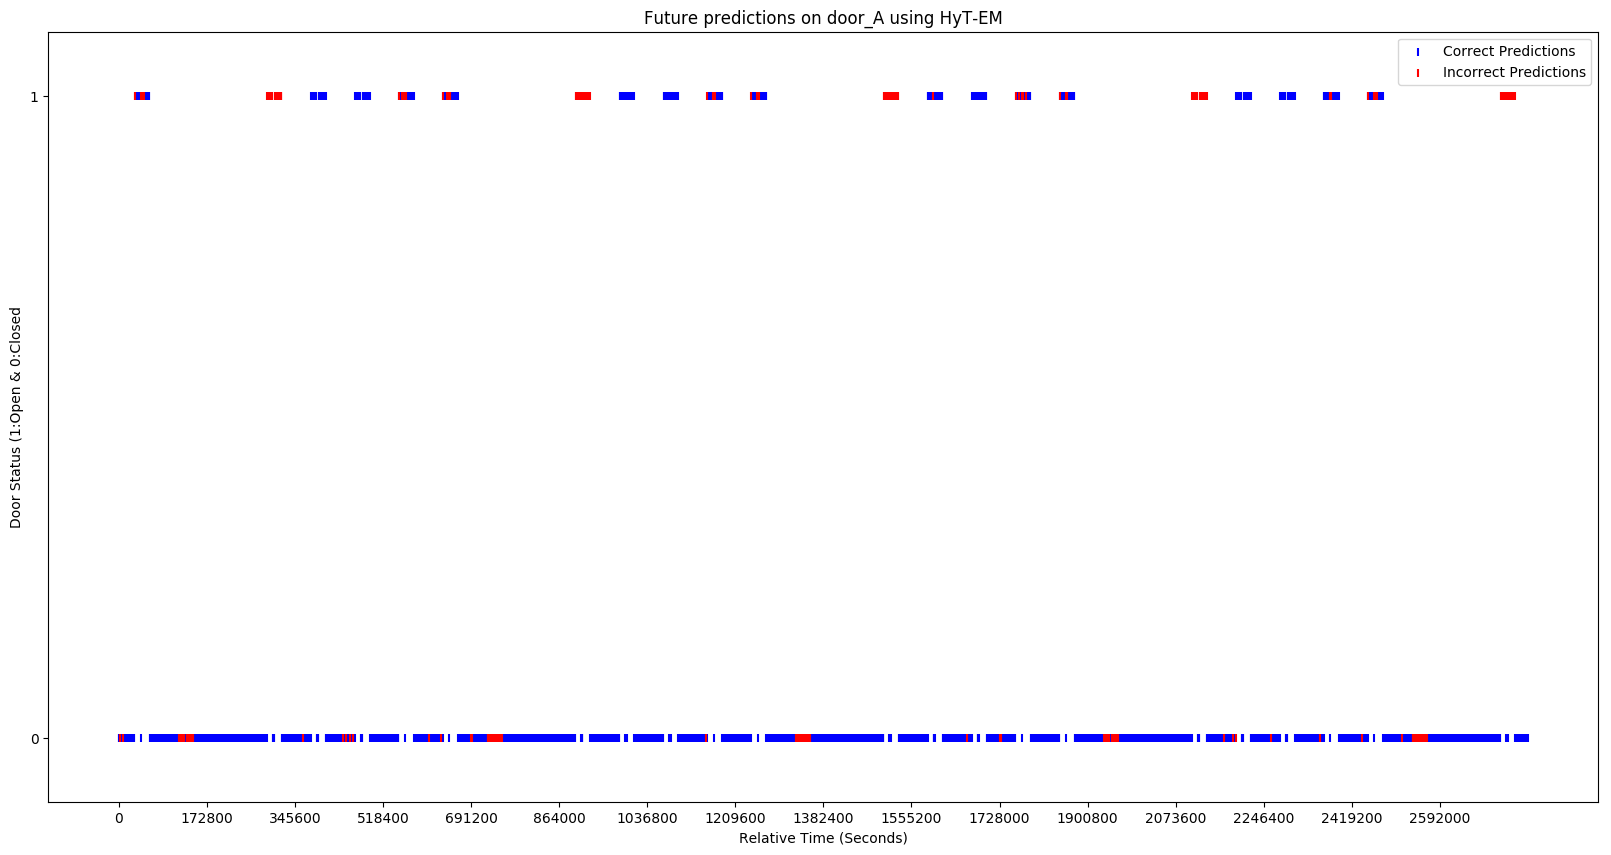
\includegraphics[width = 3in]{images/results/Future_door_A_HyT-EM.png}} \\
  \end{tabular}
  \caption{Future Predictions - Door A}
\end{figure} \\ \\

\begin{figure}
  \begin{tabular}{cc}
    {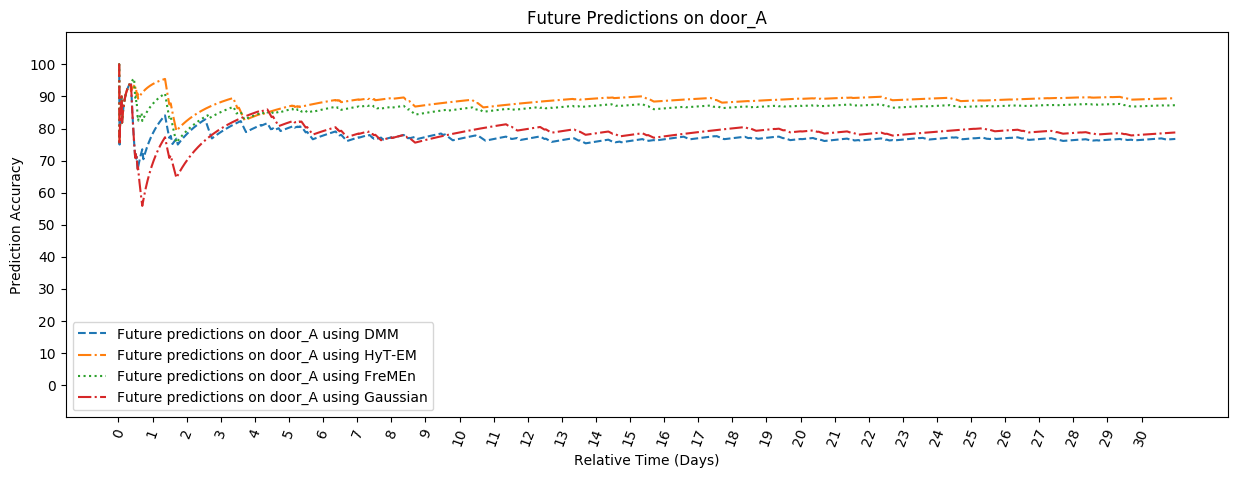
\includegraphics[width = 3in]{images/results/Future_Predictions_on_door_A.png}} &
    {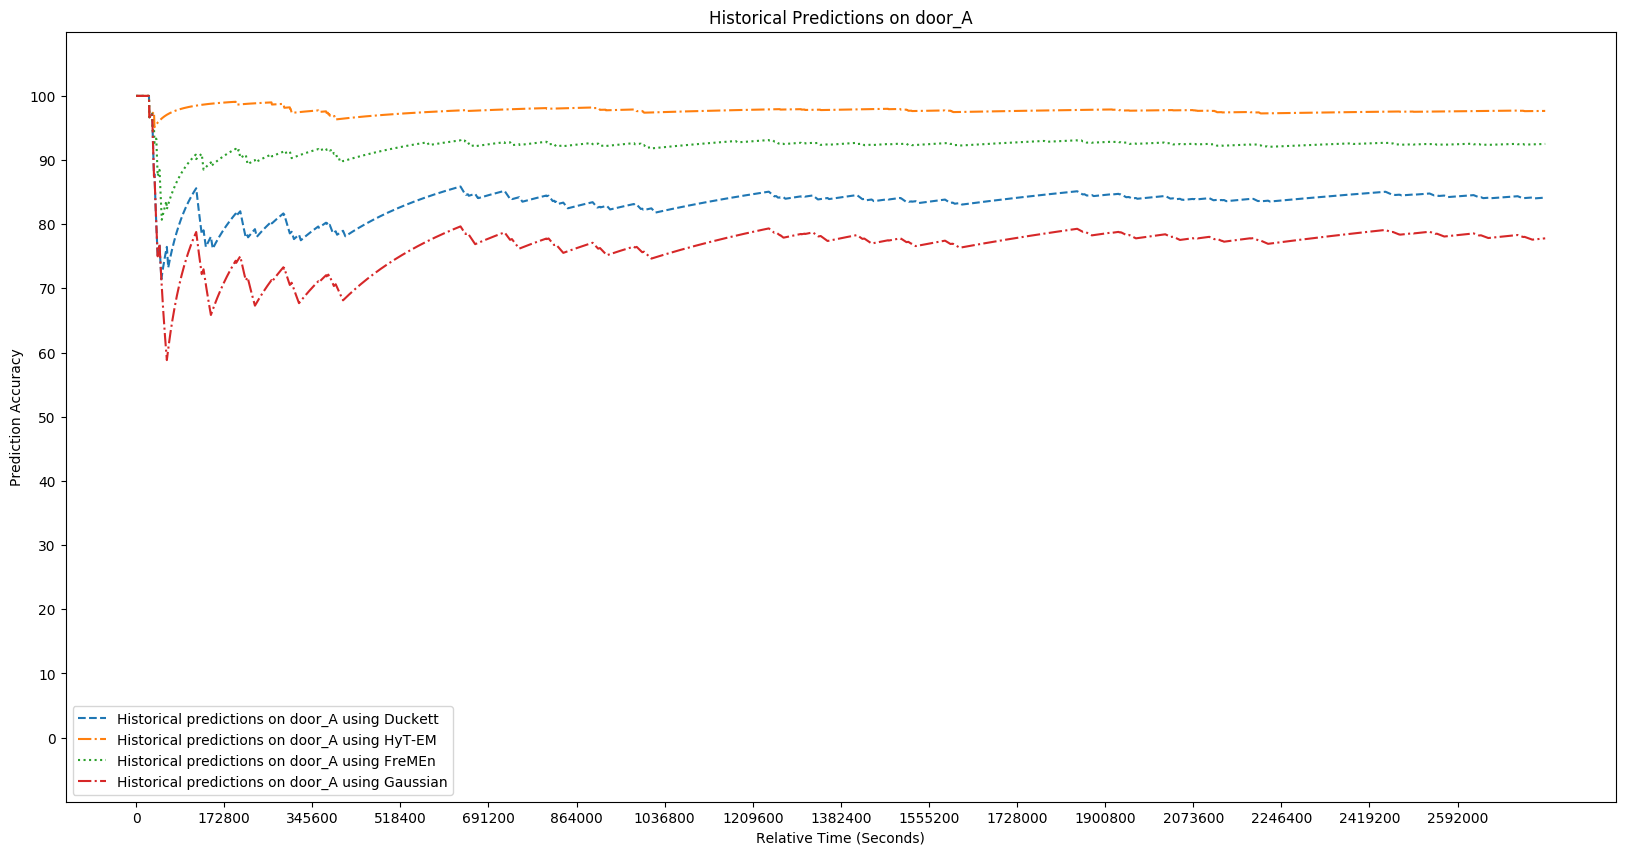
\includegraphics[width = 3in]{images/results/Historical_Predictions_on_door_A.png}} \\
  \end{tabular}
  \caption{Model Accuracy Over Time - Door A}
\end{figure} \\ \\

\subsection { Door B }

Door B demonstrates a fact the will be come increasingly clear with future
experiments.  Methods that use a modified version of the Fourier transform as
described in TODO: CITATION require a certain threshold of frequency to be met
in order to accurately predict.  In fact, it's interesting to note that the
very thing that allows these methods perform so well with periodic behavior
causes issues with datasets with non periodic behavior or datasets with
minimal periods of periodic data. \\

\begin{table}[h!]
  \centering
  \resizebox{\textwidth}{!}{%
    \begin{tabular}{|l|l|l|l|l|}
      \hline
      & Duckett & Gaussian & FreMEn  & HyperTime \\ \hline
      Historical Accuracy             & 85.71\% & 59.81\%  & 75.20\% & 71.55\%   \\ \hline
      Prediction Accuracy             & 69.24\% & 62.17\%  & 76.95\% & 75.78\%   \\ \hline
      Computation Time (Milliseconds) & 600     & 60       & 80      & 1440      \\ \hline
      Memory Usage (KB)               & 31036   & 34644    & 34892   & 37692     \\ \hline
    \end{tabular}%
  }
  \caption{Door B Data Overview}
\end{table} \\

Duckett, relying almost solely on averages, does surprisingly well on this
experiment beating out all other models in both historical and prediction
accuracy.  It is, however, important to note the flaws in Duckett's long-term
prediction. Due to the fact that future predictions are not directly possible
using Duckett and thus previous month data is used, it is clear to see that
while Duckett performed overall well historically, it is not without problems
in future prediction.  Of particular interest is its failure to continue to
accurately predict a periodic behavior that does not occur on month
boundaries. Since the behavior that happens every three days does not happen
on the same day between the two months Duckett incorrectly predicts its
occurrence as happening on the same days as last month.

In terms of resource usage, a similar trend to door A is observed. Gaussian
and FreMEn predictions take under 100 milliseconds while Duckett takes around
an order of magnitude longer, and HyperTime yet another order of magnitude
longer. Finally, similar to door A, all approaches use about the same amount
of memory for training and predicting using around 30 megabytes while being
within about 10 megabytes of one another.

\begin{figure}
  \begin{tabular}{cc}
    {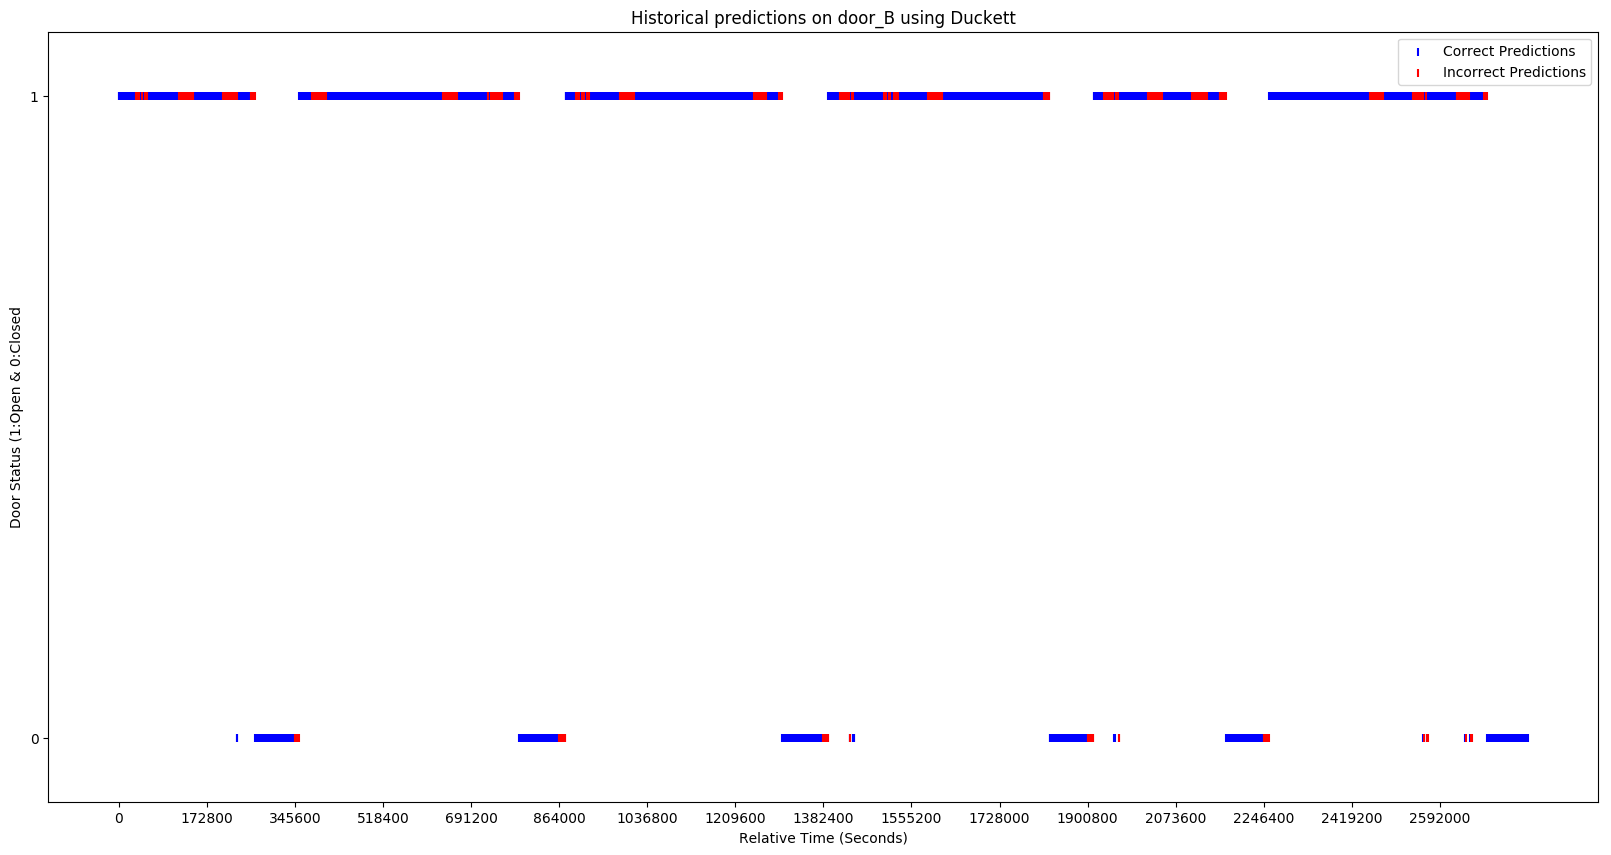
\includegraphics[width = 3in]{images/results/Historical_door_B_Duckett.png}} &
    {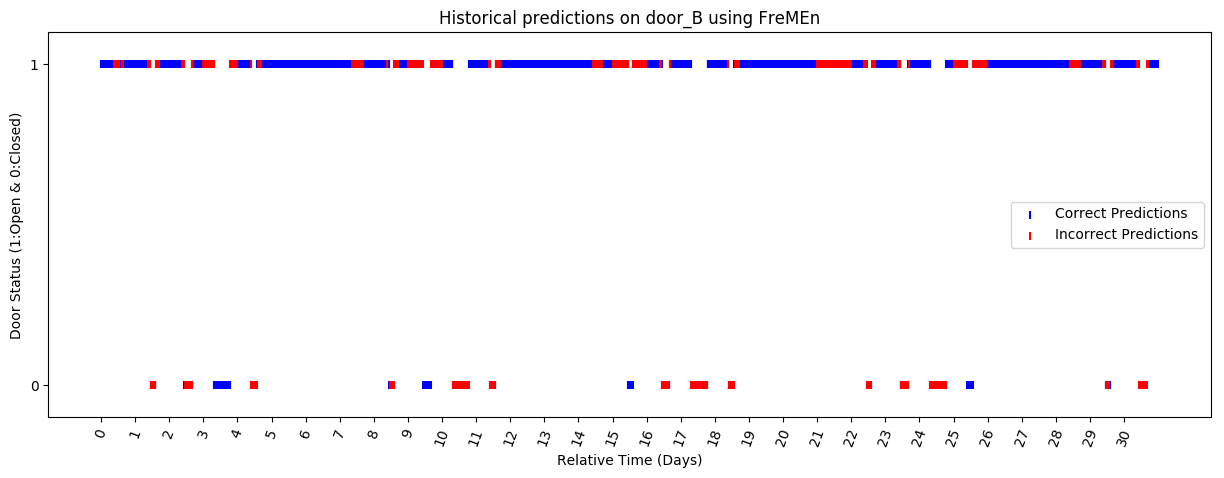
\includegraphics[width = 3in]{images/results/Historical_door_B_FreMEn.png}} \\
    {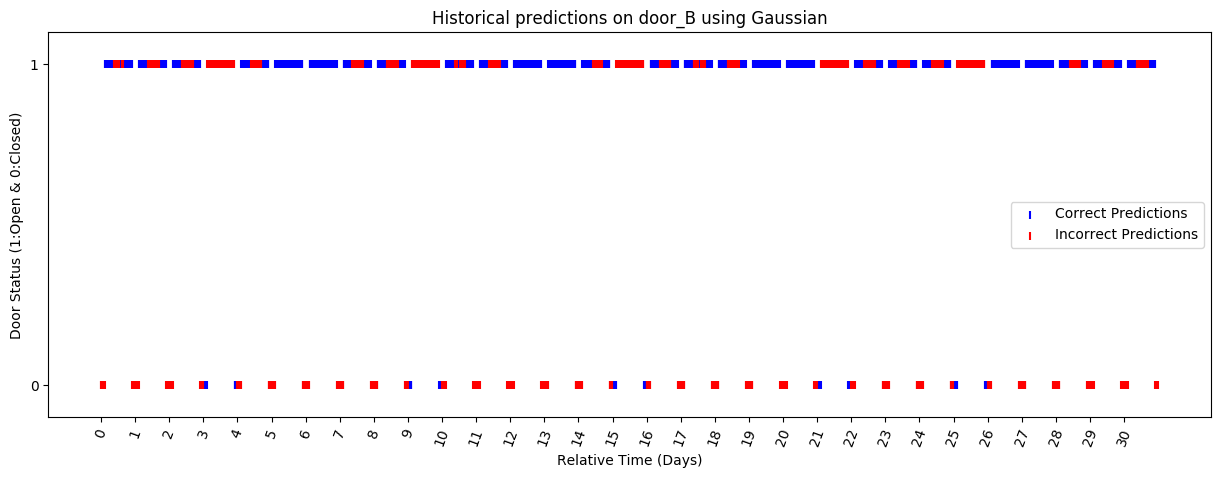
\includegraphics[width = 3in]{images/results/Historical_door_B_Gaussian.png}} &
    {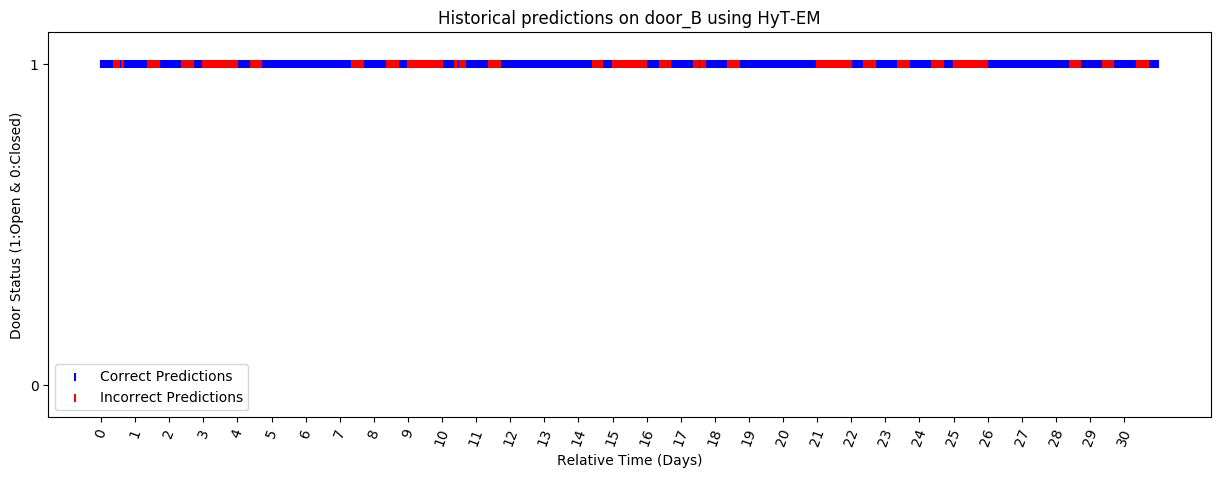
\includegraphics[width = 3in]{images/results/Historical_door_B_HyT-EM.png}} \\
  \end{tabular}
  \caption{Historical Recreations - Door B}
\end{figure}\\ \\

\begin{figure}
  \begin{tabular}{cc}
    {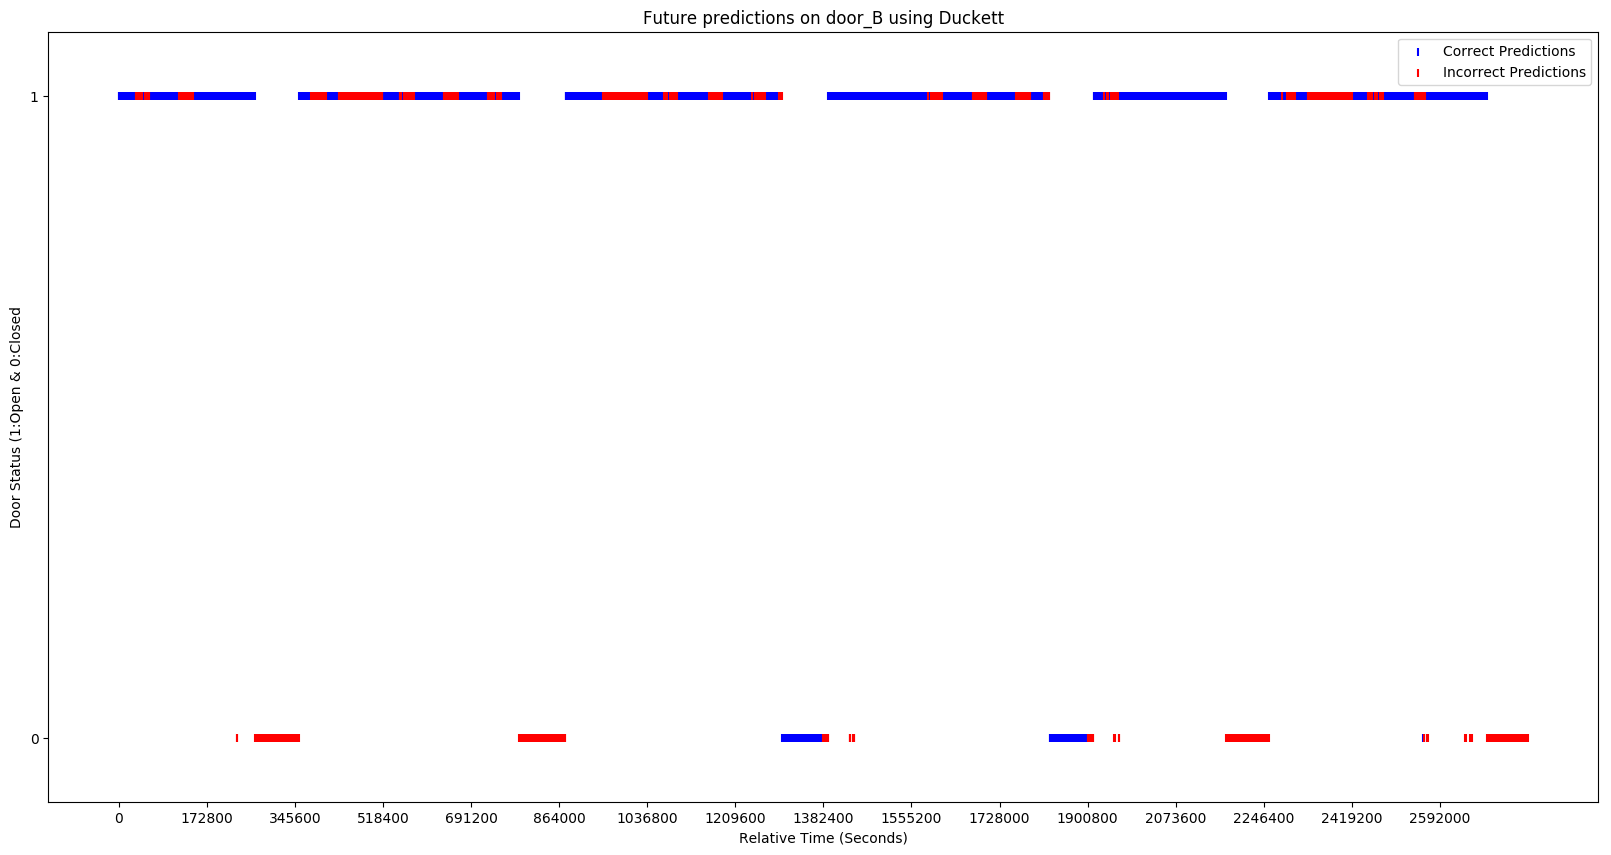
\includegraphics[width = 3in]{images/results/Future_door_B_Duckett.png}} &
    {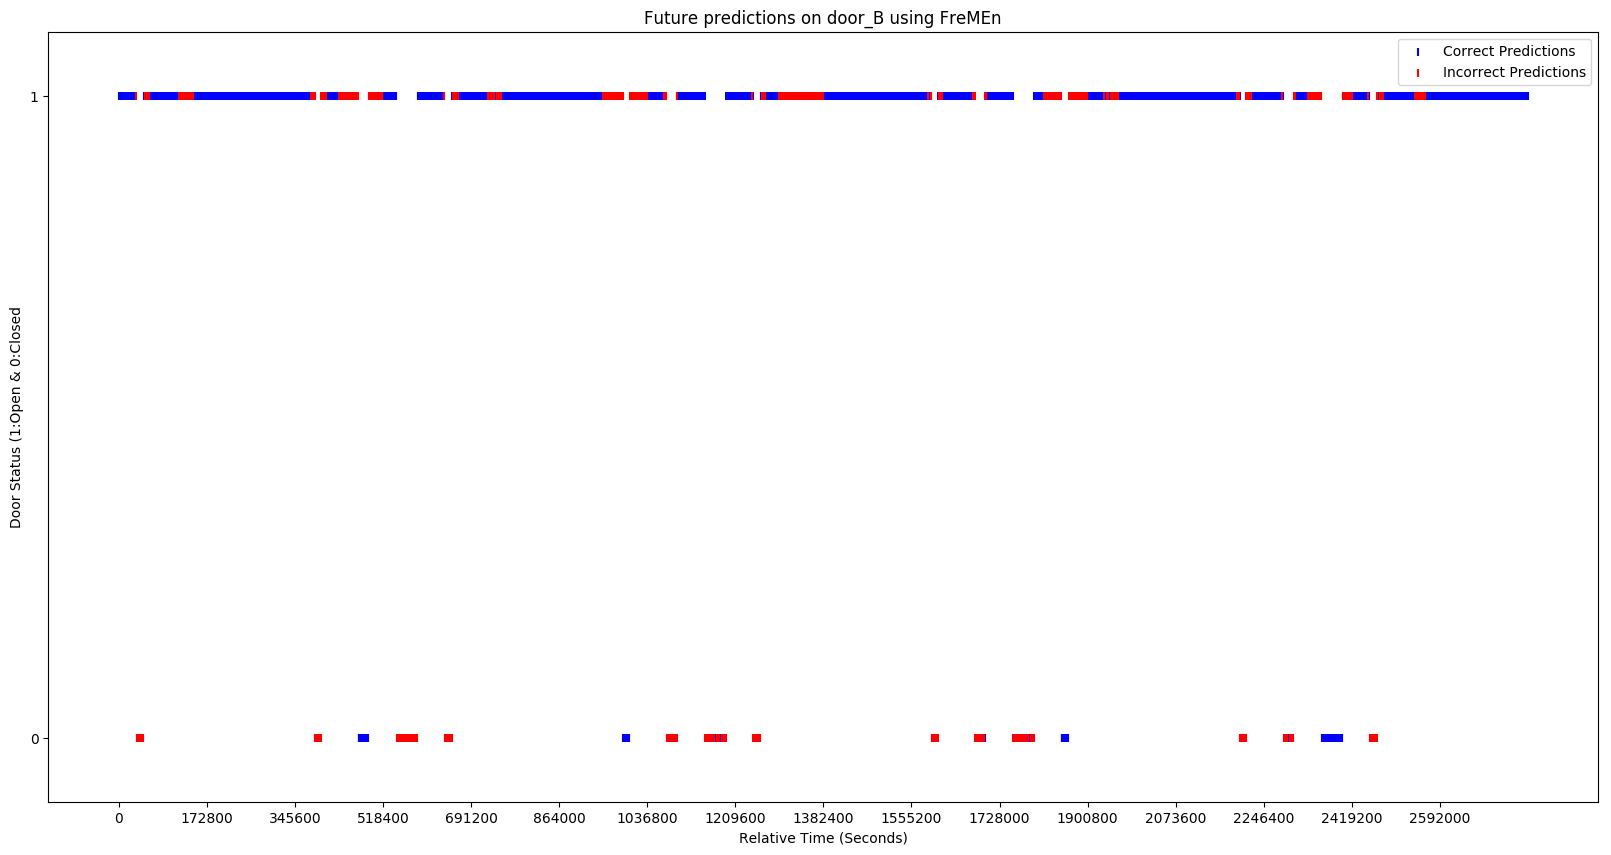
\includegraphics[width = 3in]{images/results/Future_door_B_FreMEn.png}} \\
    {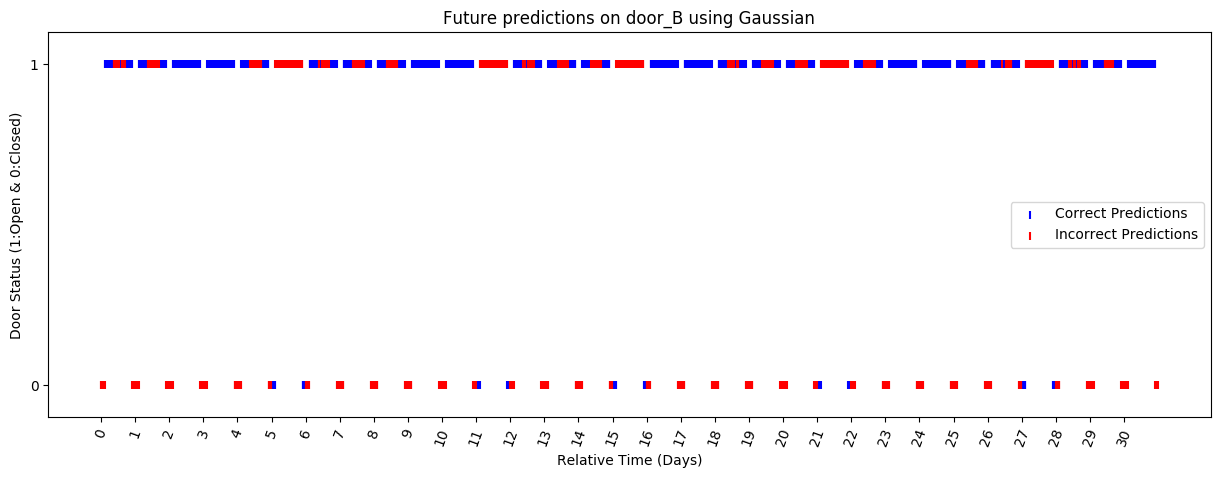
\includegraphics[width = 3in]{images/results/Future_door_B_Gaussian.png}} &
    {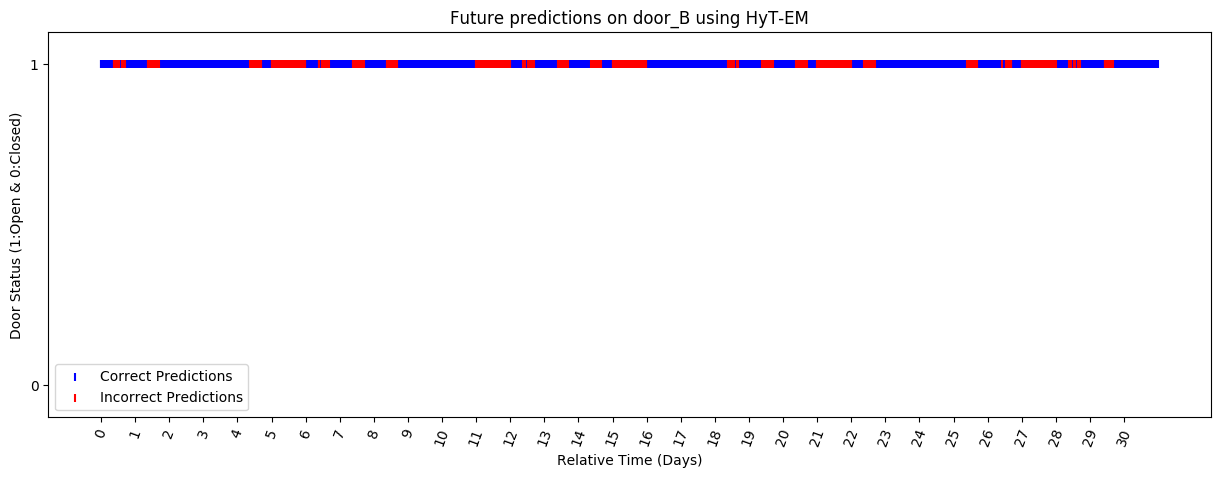
\includegraphics[width = 3in]{images/results/Future_door_B_HyT-EM.png}} \\
  \end{tabular}
  \caption{Future Predictions - Door B}
\end{figure}\\ \\

\begin{figure}
  \begin{tabular}{cc}
    {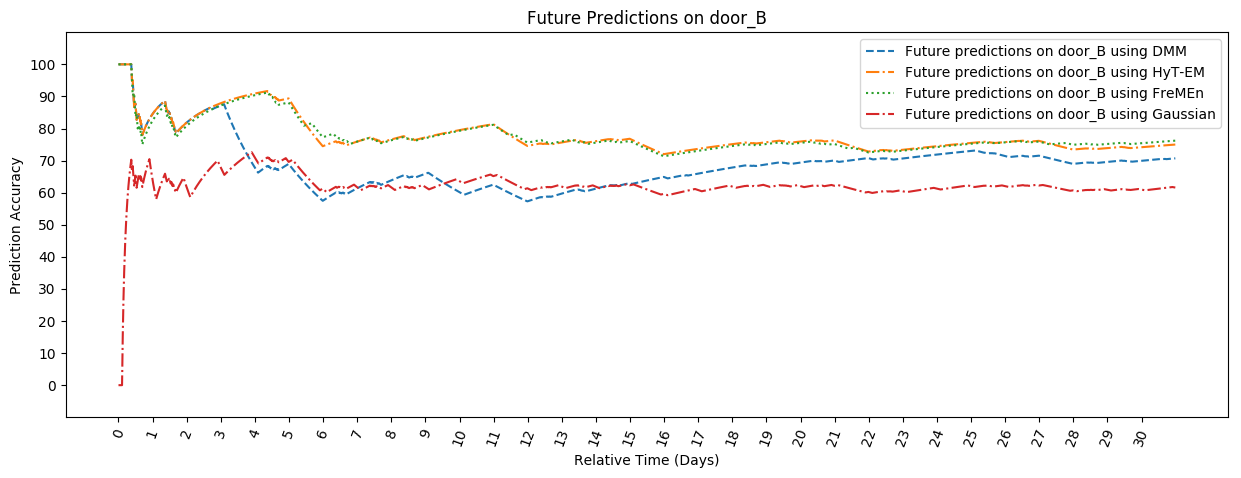
\includegraphics[width = 3in]{images/results/Future_Predictions_on_door_B.png}} &
    {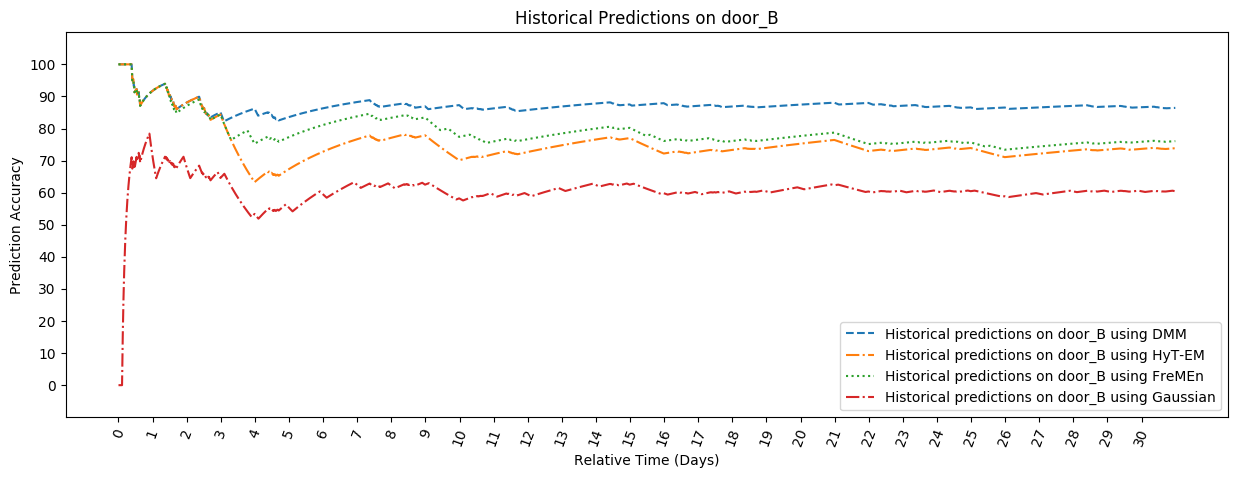
\includegraphics[width = 3in]{images/results/Historical_Predictions_on_door_B.png}} \\
  \end{tabular}
  \caption{Model Accuracy Over Time - Door B}
\end{figure}\\ \\



\subsection { Door C }

With door A exemplifying the occasionally periodic and somewhat noisy
behaviour in the real world, door C serves as almost the exact opposite,
modeling a one time, long-term change.
Perhaps some what expectedly, the results in terms of prediction accuracy are
almost completely opposite that of door A with Duckett having the best
performance both historically and with future predictions. \\

Unfortunately, despite its better performance by the numbers in table 6.3,
looking at the resulting graphs in table 6.7 and 6.8 shows a somewhat
initially disappointing result. As discussed in the door B experiment,
Duckett, merely uses it's historically prediction again for future
predictions. This is clearly visible by the prediction of the door being open
for the first three weeks in the future predictions.  However, Duckett was not
designed for long-term future predictions and instead meant to be used
``live''. When this is accounted for, Duckett's performance is once again
impressive.  In fact, as discussed TODO: where will this be discussed? the
historical predictions made by Duckett can be view as it's ``live''
predictions and thus it would be expected that in the real world it would
continue to predict the door as being closed as long as long-term future
predictions are not requested. This means that it is likely Duckett's
performance would be closer to 100\% for future actives for as long as the door
remained shut. \\

\begin{table}[h!]
  \centering
  \resizebox{\textwidth}{!}{%
    \begin{tabular}{|l|l|l|l|l|}
      \hline
      & Duckett & Gaussian & FreMEn  & HyperTime \\ \hline
      Historical Accuracy             & 99.56\% & 62.75\%  & 67.74\% & 67.74\%   \\ \hline
      Prediction Accuracy             & 31.82\% & 14.58\%  & 00.00\% & 00.00\%   \\ \hline
      Computation Time (Milliseconds) & 570     & 60       & 70      & 530       \\ \hline
      Memory Usage (KB)               & 31224   & 35004    & 34976   & 37208     \\ \hline
    \end{tabular}%
  }

  \caption{Door C Data Overview}
\end{table}

As alluded to above in door B's experiment, the lack of periodic data has
caused both FreMEn and HyperTime to take the easiest prediction for the
training data and predict that the door will always be open. Unfortunately,
this causes the future predictions to be entirely inaccurate. The only possible redemption
for the Fourier based approaches on this long term changes is that the
prediction would eventually flip to always being closed, but only after the total number of observations of the door being
closed surpassed that of the door being open. In this case, that would take a
total of just over 6 weeks if training was being done every night. \\

The resource usage statistics in figure 6.3 do interestingly break slightly
from the norm. It appears that due to the simplistic predictions of the
Fourier approaches, HyperTime has shaved off an order of magnitude in
computation time. This is believed to be because the prediction model created
by HyperTime, after the initial naive approach, has a larger error than the first and thus it immediately quits
and stops attempting to improve the model. This is irrelevant however, seeing
as the predictions are completely inaccurate so any gain in computational time
is meaningless.

\begin{figure}
  \begin{tabular}{cc}
    {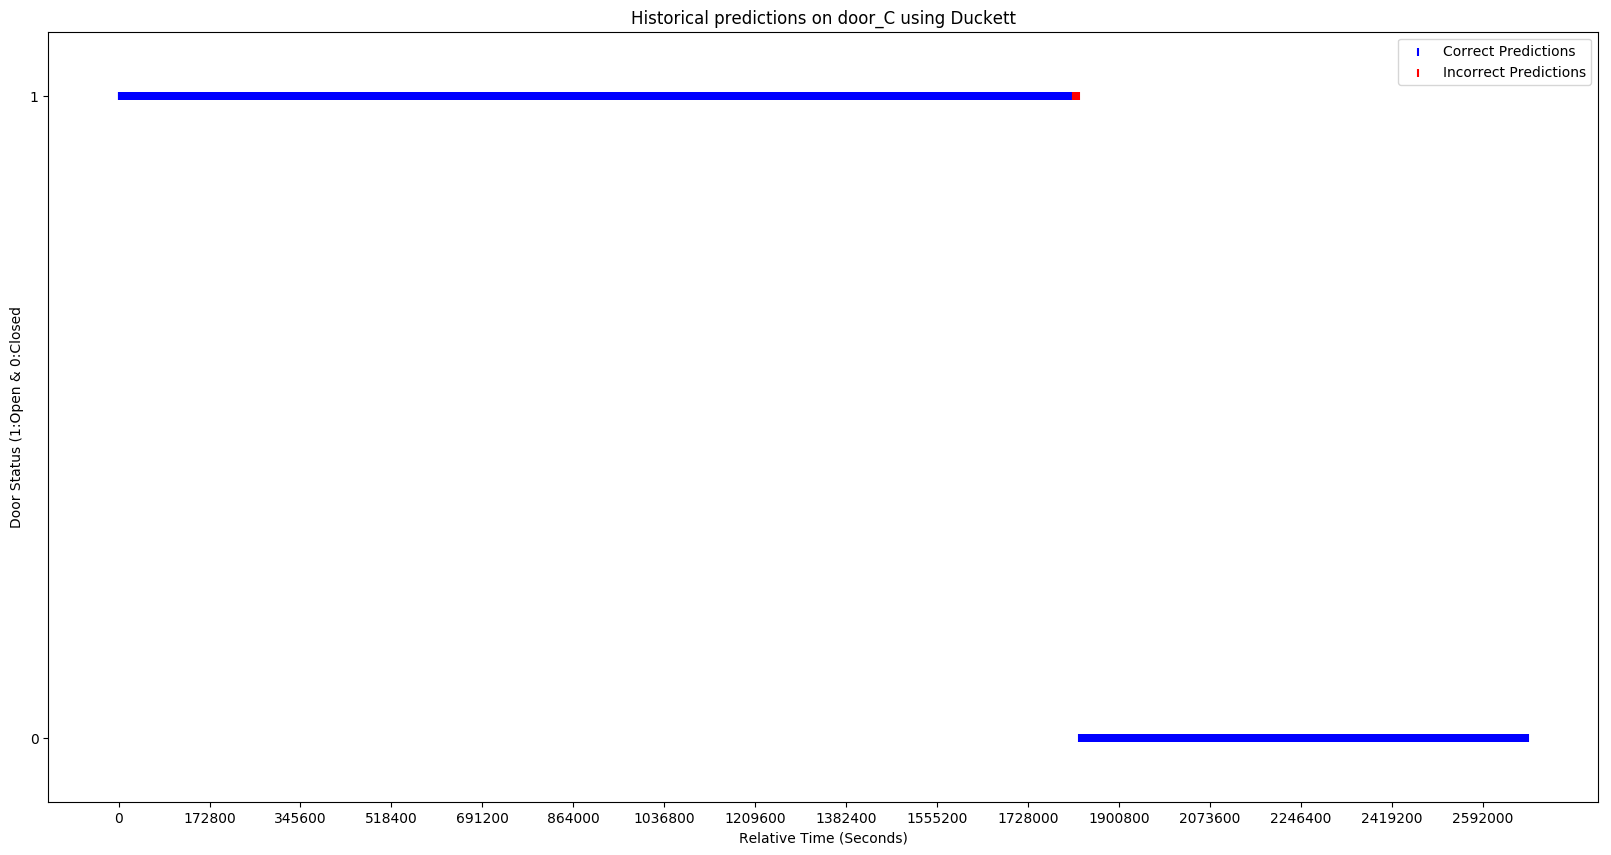
\includegraphics[width = 3in]{images/results/Historical_door_C_Duckett.png}} &
    {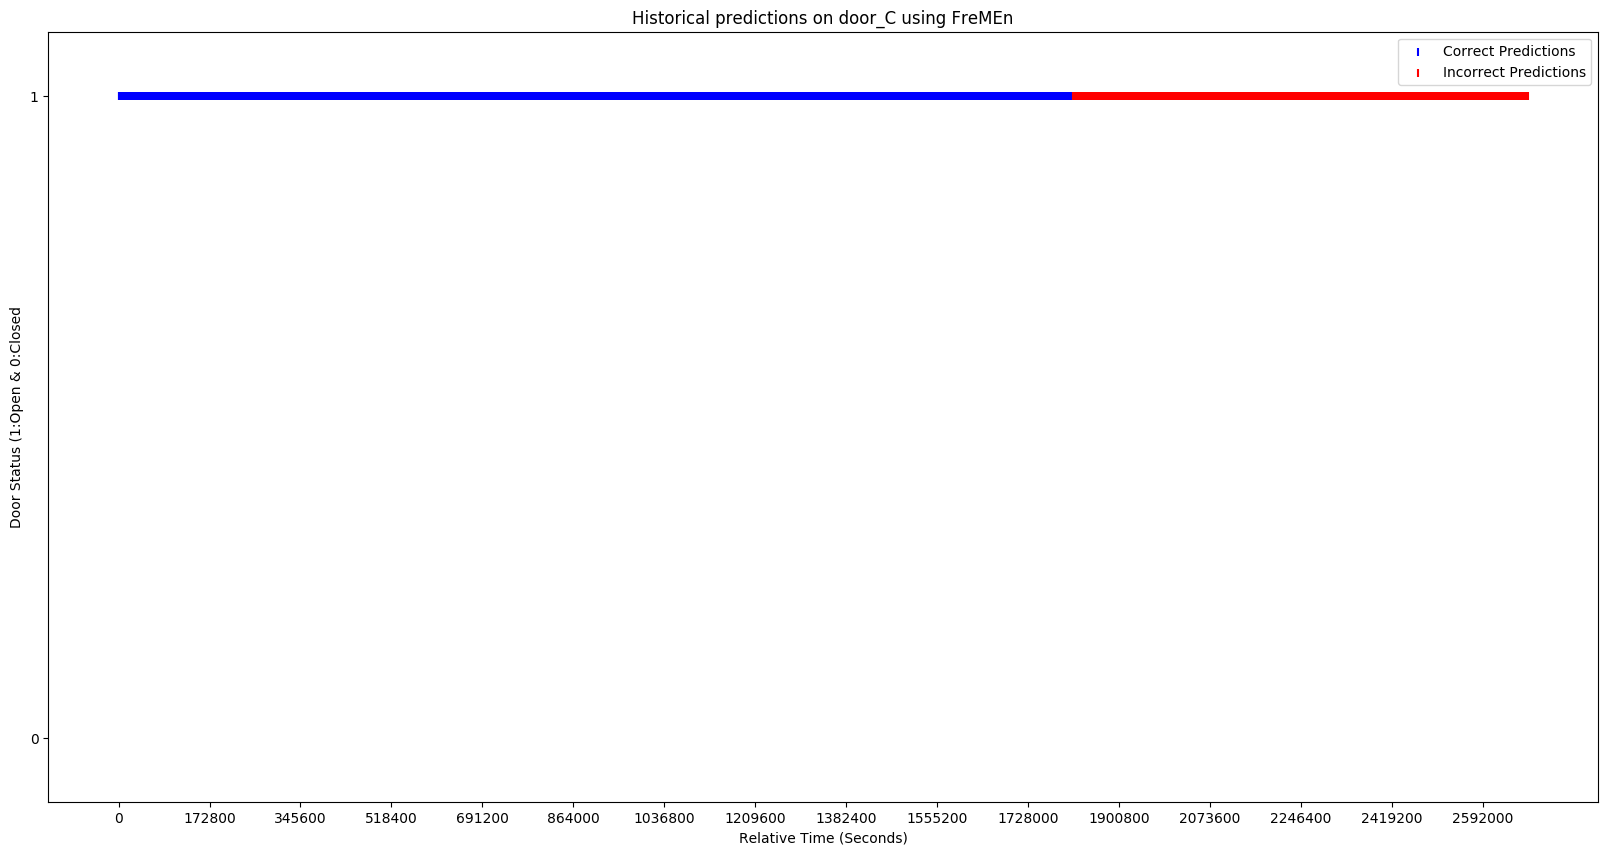
\includegraphics[width = 3in]{images/results/Historical_door_C_FreMEn.png}} \\
    {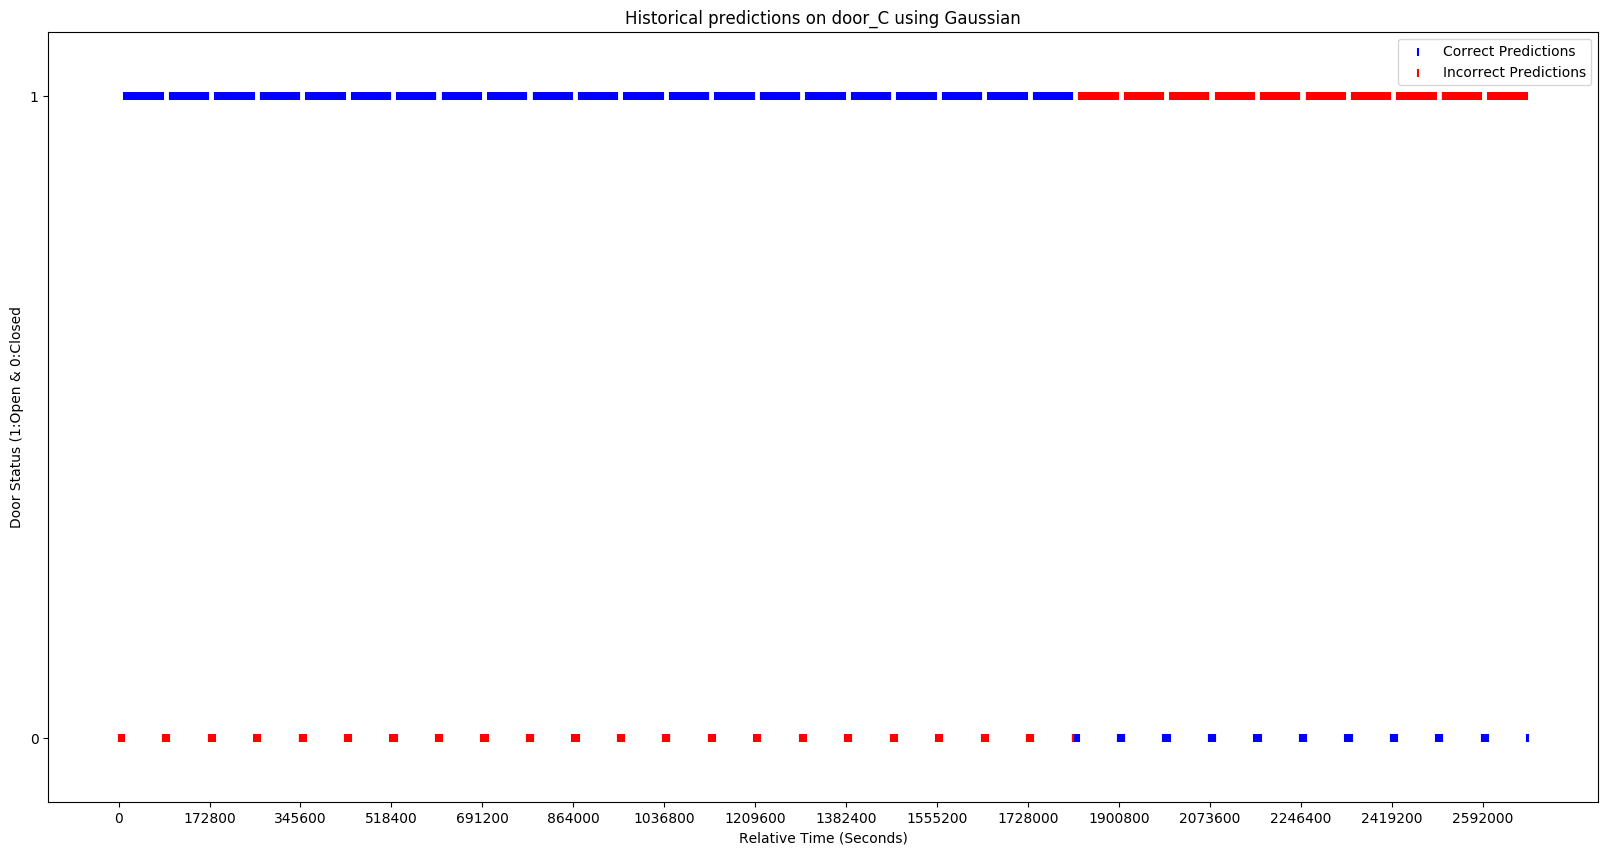
\includegraphics[width = 3in]{images/results/Historical_door_C_Gaussian.png}} &
    {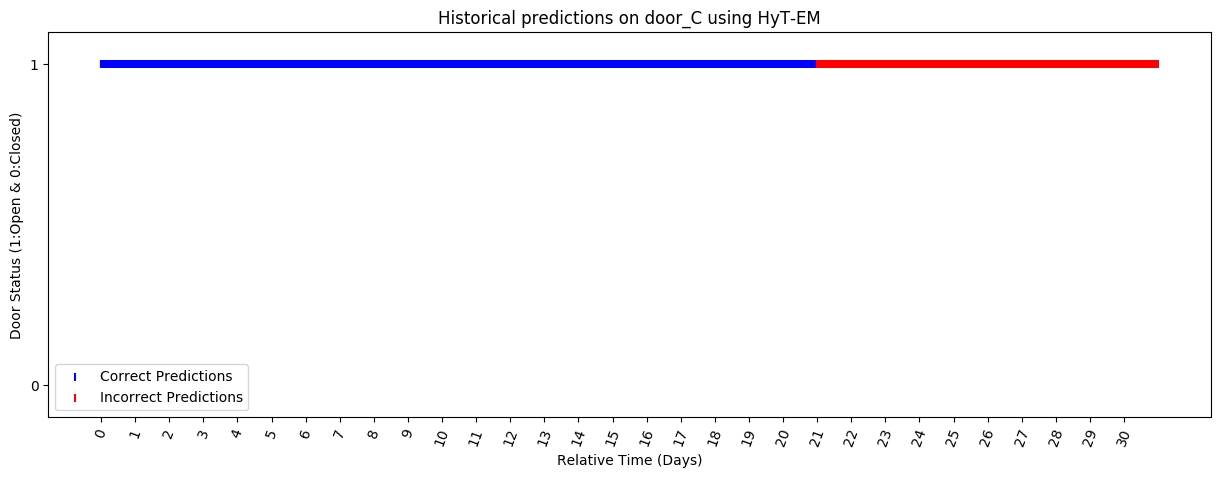
\includegraphics[width = 3in]{images/results/Historical_door_C_HyT-EM.png}} \\
  \end{tabular}
  \caption{Historical Recreations - Door C}
\end{figure}\\ \\

\begin{figure}
  \begin{tabular}{cc}
    {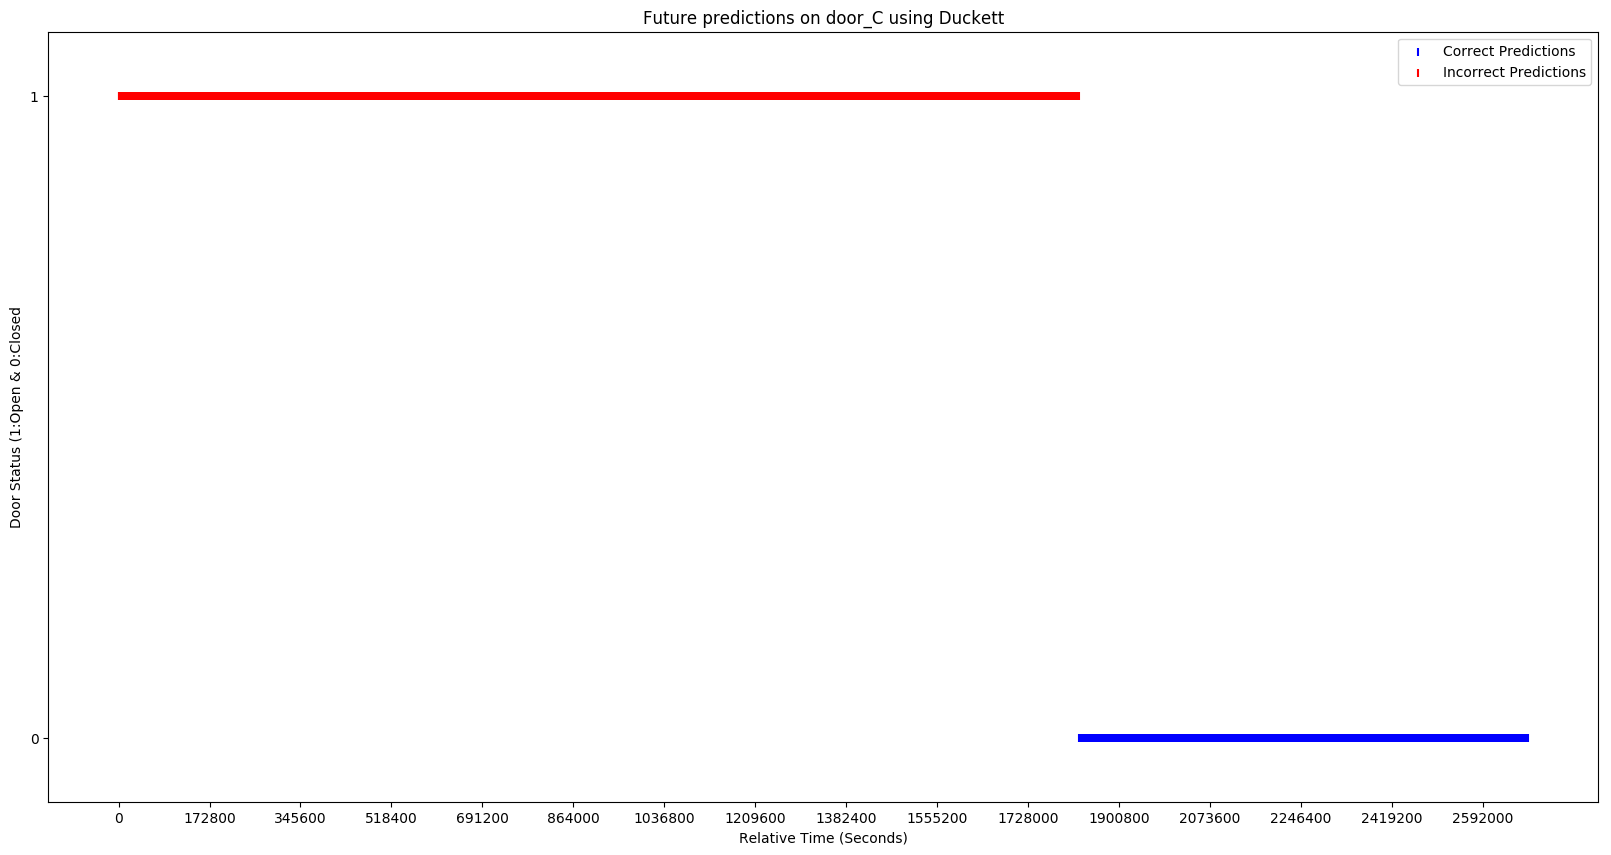
\includegraphics[width = 3in]{images/results/Future_door_C_Duckett.png}} &
    {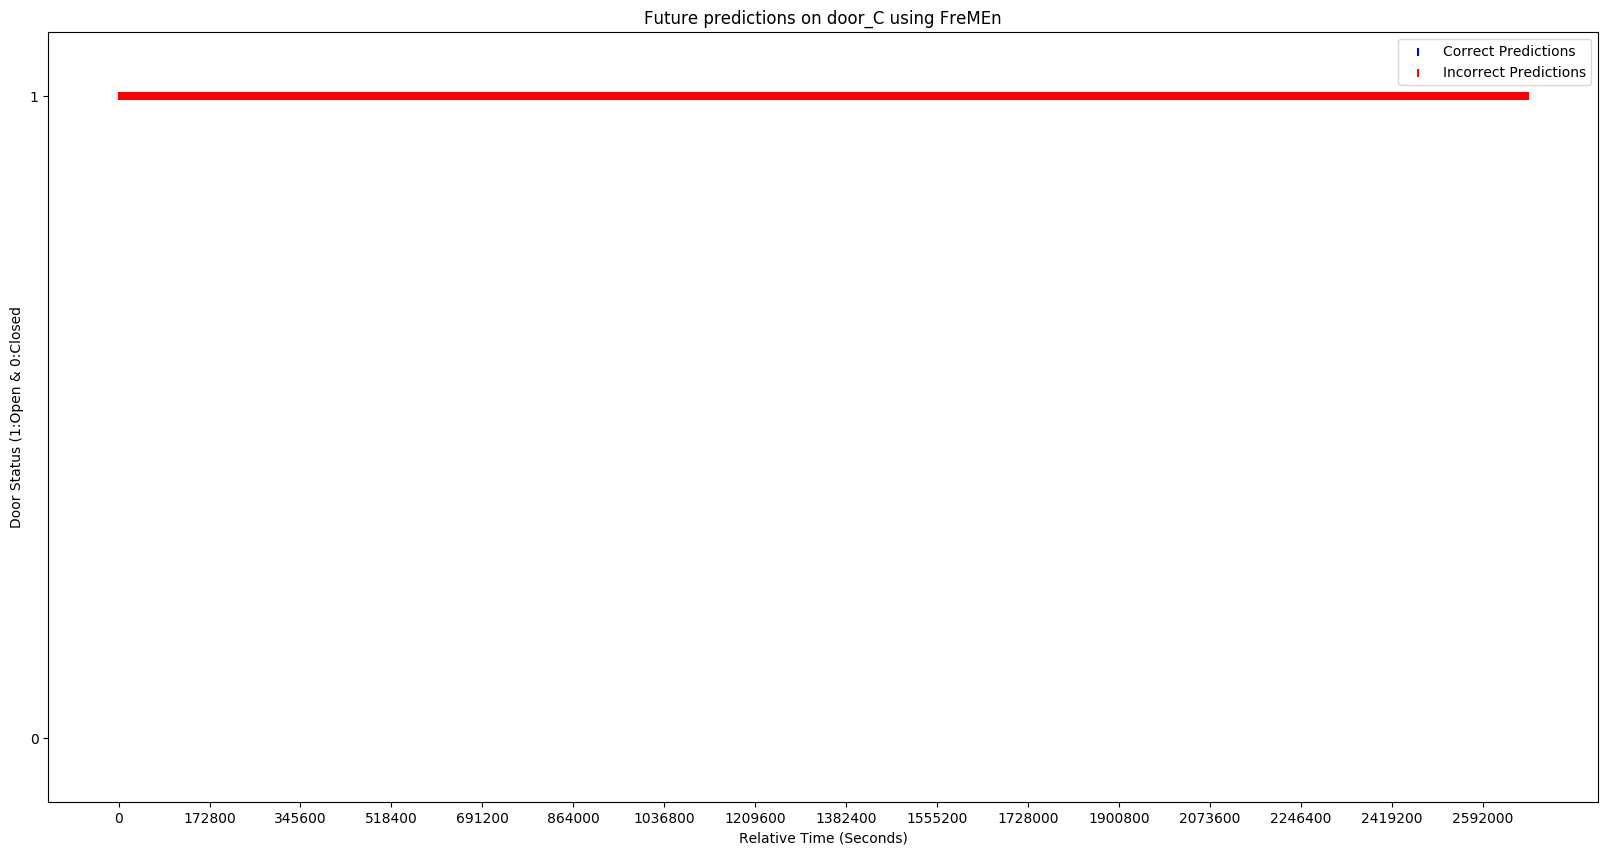
\includegraphics[width = 3in]{images/results/Future_door_C_FreMEn.png}} \\
    {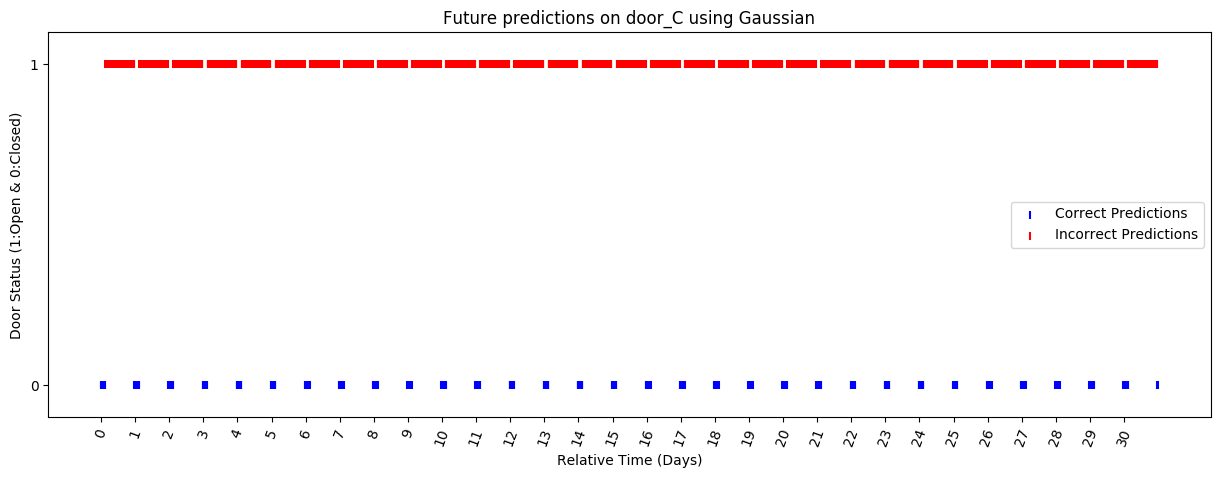
\includegraphics[width = 3in]{images/results/Future_door_C_Gaussian.png}} &
    {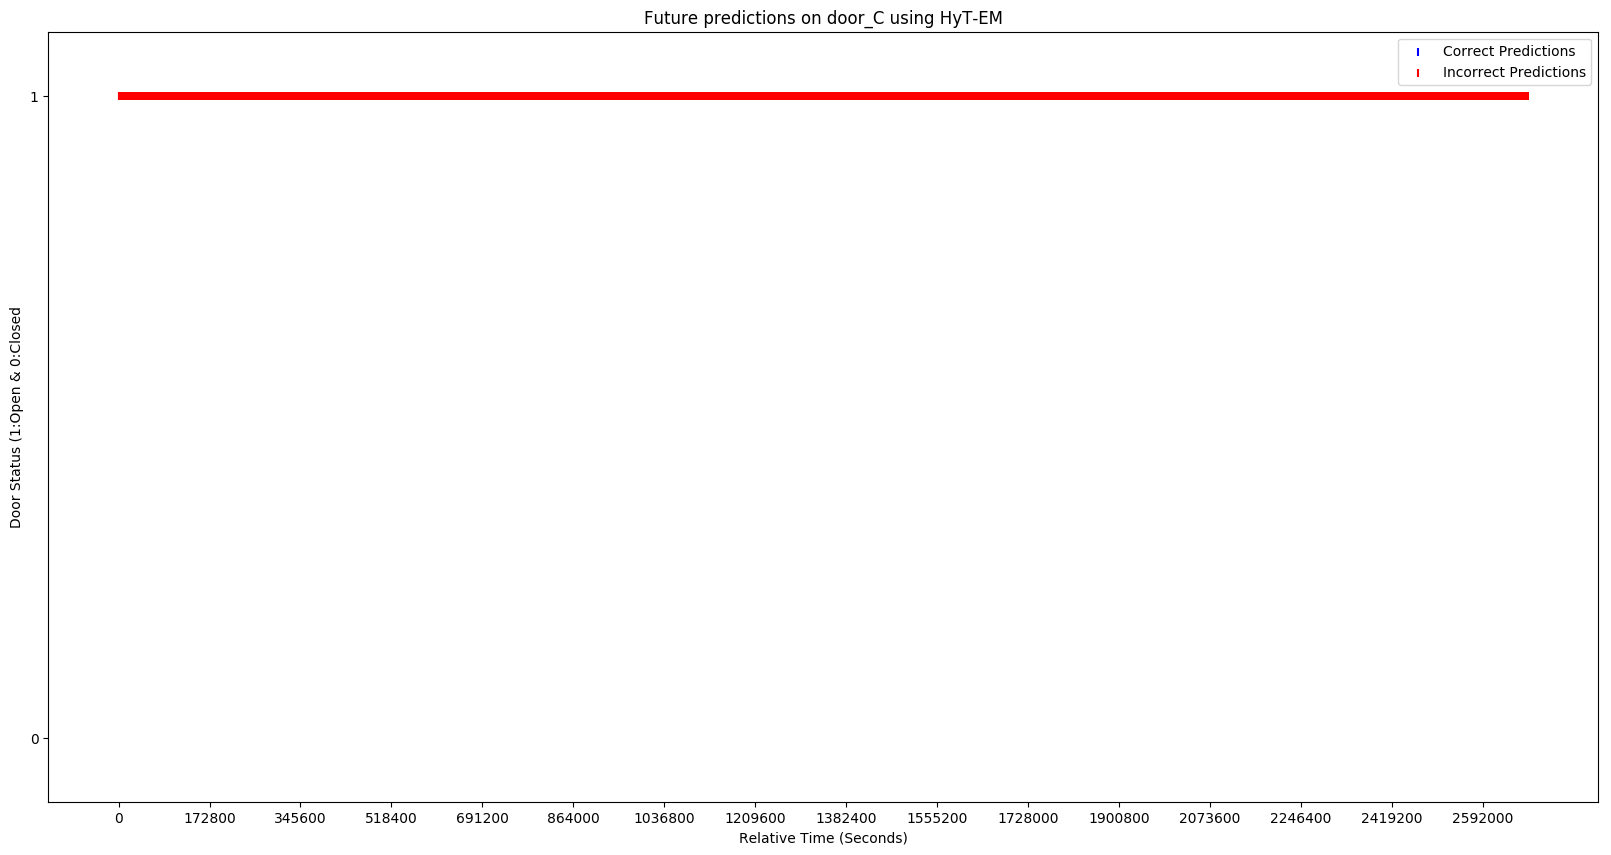
\includegraphics[width = 3in]{images/results/Future_door_C_HyT-EM.png}} \\
  \end{tabular}
  \caption{Future Predictions - Door C}
\end{figure}\\ \\

\begin{figure}
  \begin{tabular}{cc}
    {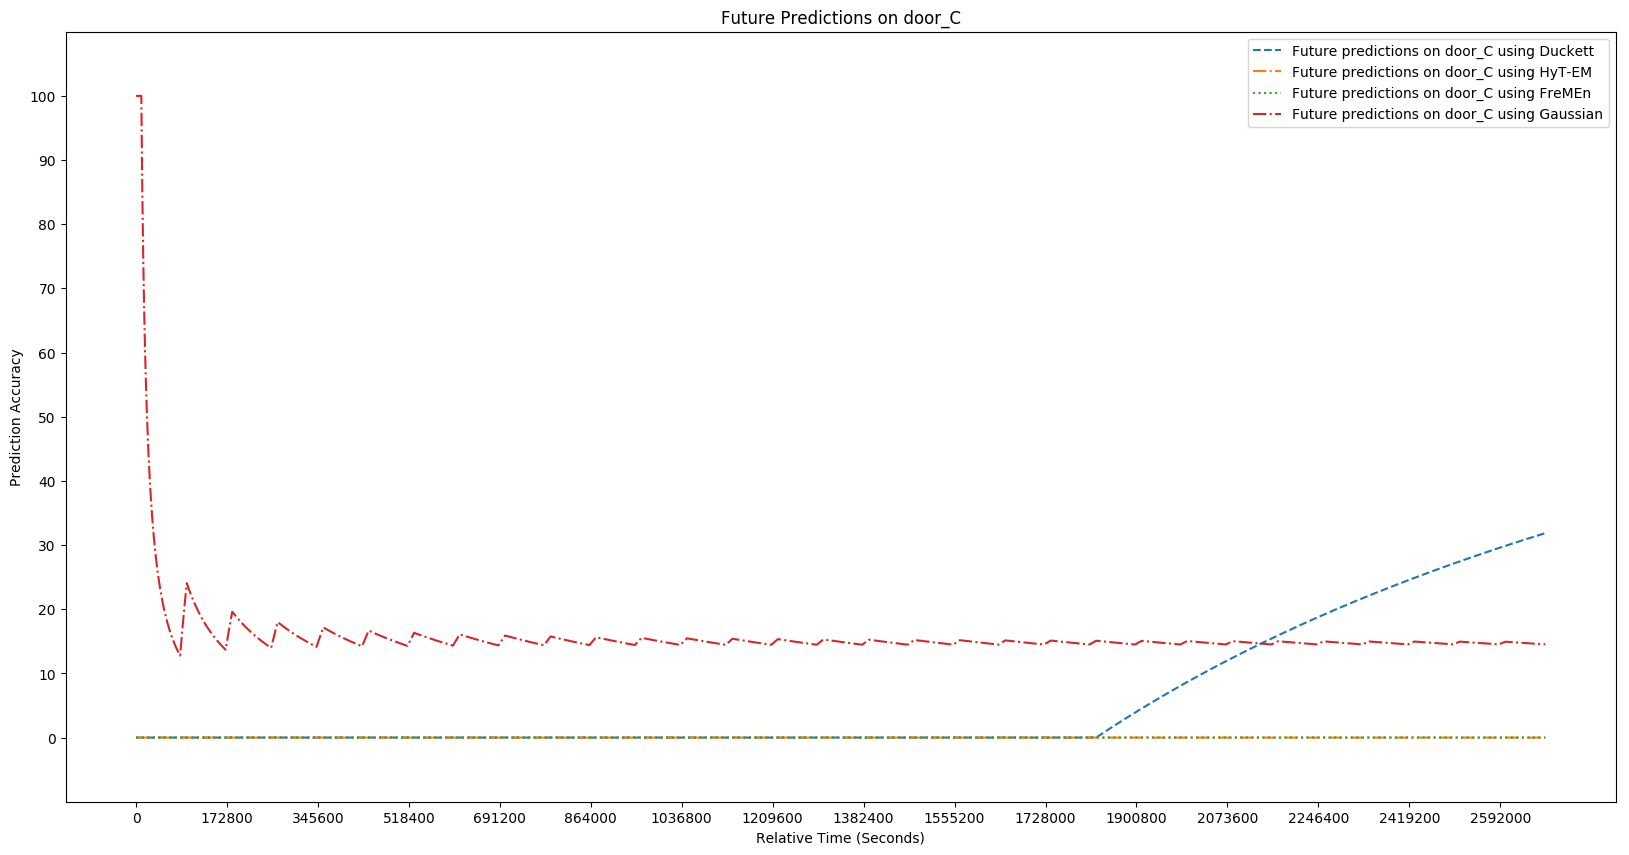
\includegraphics[width = 3in]{images/results/Future_Predictions_on_door_C.png}} &
    {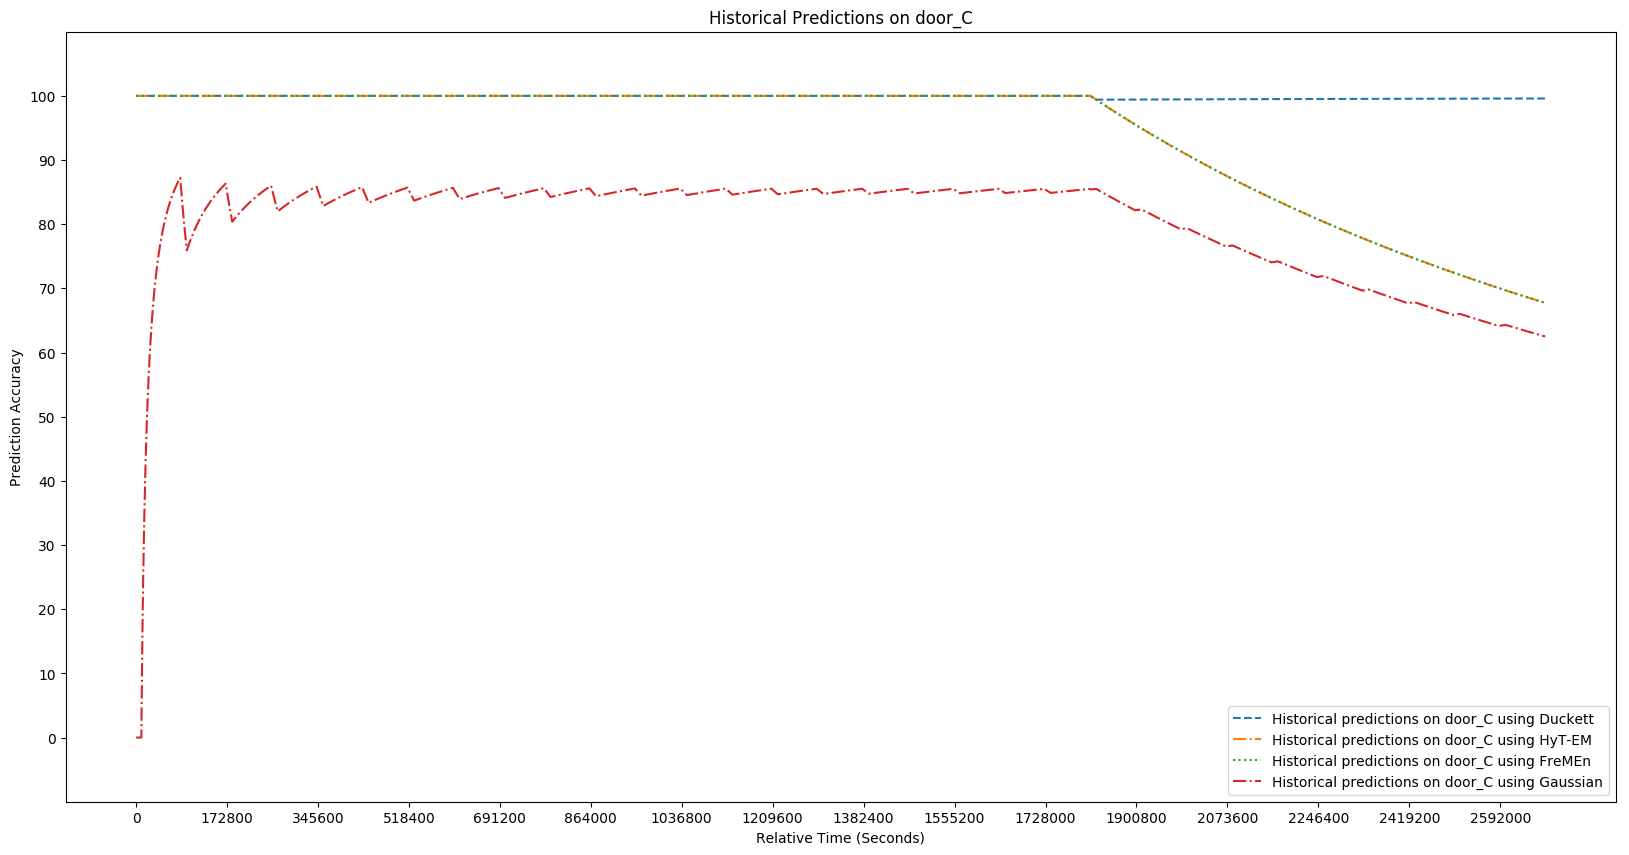
\includegraphics[width = 3in]{images/results/Historical_Predictions_on_door_C.png}} \\
  \end{tabular}
  \caption{Model Accuracy Over Time - Door C}
\end{figure}\\ \\


\section{ Congested Hallways }
TODO pair down images and move them to the end of the paper

Having already given an in depth look at the individual predictions in the
previous section, this section will not focus on detailing every methods results on every data set,
but instead focus on meta information that can be abstracted as well as
performance with respect to path planning, the ultimate use goal.
To this effect, although graphs for every single result are not
present in this section they are available in TODO WHATS THE SECTION CALLED? \\

\subsection{ Prediction Accuracy Versus Behavior Frequency }
TODO list figures where these numbers can be found ?
TODO add talk about the same mistake in hypertime on trash

With a moderately size set that has varying frequencies such as the one
described above, it is possible to observe a relationship between the accuracy
of a given spatio-temporal modeling technique and the period of the behavior
attempting to be modeled. In general, that data suggest that behaviors with
a higher frequency are better modeled using Fourier methods like FreMEn and
HyperTime. This is most obvious when looking at behaviors that repeated multiple
times a day such as the laundry or meal nodes. In these experiments the Fourier
methods achieved an impressive 100\% accuracy. TODO should this go here or
else where\?  One caveat to these impressive results is the lack of noise
present in the data used for the hallway test. Large amounts of noise were
explicitly left out of this particular experiment in to minimize the variables
present. The presence and effect of noise in data is, however, analyzed in
both the door and elevator experiments. \\

\begin{table}[h!]
  \centering
  \resizebox{\textwidth}{!}{%
    \begin{tabular}{|l|l|l|l|l|}
      \hline
      & Duckett & Gaussian & FreMEn  & HyperTime \\ \hline
      Historical Accuracy             & 78.93\% & 26.04\%  & 100.00\% & 100.00\% \\ \hline
      Prediction Accuracy             & 78.93\% & 26.04\%  & 100.00\% & 100.00\% \\ \hline
      Computation Time (Milliseconds) & 610     & 60       & 70       & 1860     \\ \hline
      Memory Usage (KB)               & 30984   & 35160    & 35172    & 37632    \\ \hline
    \end{tabular}%
  }
  \caption{Hallway Laundry Section}
\end{table}

\begin{table}[h!]
  \centering
  \resizebox{\textwidth}{!}{%
    \begin{tabular}{|l|l|l|l|l|}
      \hline
      & Duckett & Gaussian & FreMEn  & HyperTime \\ \hline
      Historical Accuracy             & 61.63\% & 52.08\%  & 100.00\% & 100.00\% \\ \hline
      Prediction Accuracy             & 61.63\% & 52.08\%  & 100.00\% & 100.00\% \\ \hline
      Computation Time (Milliseconds) & 620     & 60       & 70       & 880      \\ \hline
      Memory Usage (KB)               & 30896   & 35524    & 35600    & 38288    \\ \hline
    \end{tabular}%
  }
  \caption{Hallway Meal Section 0}
\end{table}

\begin{table}[h!]
  \centering
  \resizebox{\textwidth}{!}{%
    \begin{tabular}{|l|l|l|l|l|}
      \hline
      & Duckett & Gaussian & FreMEn  & HyperTime \\ \hline
      Historical Accuracy             & 74.93\% & 65.62\%  & 100.00\% & 100.00\% \\ \hline
      Prediction Accuracy             & 74.93\% & 65.62\%  & 100.00\% & 100.00\% \\ \hline
      Computation Time (Milliseconds) & 600     & 60       & 70       & 990      \\ \hline
      Memory Usage (KB)               & 31384   & 35388    & 35588    & 37608    \\ \hline
    \end{tabular}%
  }
  \caption{Hallway Meal Section 1}
\end{table}


When observing the behavior that occurs with the least frequency, the trash
nodes, the opposite trend is observed. Fourier methods no longer are able to
accurately predict behaviors and their predictions drop to around 66\% accuracy.
This is not believed to be a problem predicting or modeling behaviors with a
lower frequency, but rather a consequence of the ratio between frequency and
length of observation. TODO should future work go here\? It is postulated that
with a larger data set, achievable by increasing the time of observation while
maintaining the density of observations, the predictions would improve. \\

While Fourier methods appear directly correlated with frequency, Duckett
appears to have an inverse relationship with frequency. In the meal and
laundry nodes Duckett has a prediction accuracy between around 60\% to 80\%.
Furthermore, the lowest prediction accuracy of 61.63\% is achieved on the meal
node that happens to have the highest number of changes per day. It is believed
that the poor behavior of Duckett on behaviors with high frequency is due to
how the averages are stored and computed. The method undergoes a type of
trashing where in by the time the model has adjusted to current state of a
behavior the behavior changes. It is important to note, that if prior knowledge
or a previous data set is known, the model parameters such as refresh rate TODO
correct terminology? can be tuned to best fit the frequency of a given behavior.
However, this would have to be done for ever behavior, or at least a set or class
of given behaviors and there currently does not exist a method to do this
automatically or on a large scale. One final note about Duckett's performance
with respect to frequency, similar to what happened in the door B experiment,
Duckett fails to accurately predict behaviors that have periods that do not
fall on month boundaries. This is visible in the difference between historical
and future prediction accuracy for the trash sections dropping as far as from
91.13\% to 32.13\% in the trash 0 node. Once again, this is not a direct failure
of the Duckett model itself, but a result of forcing Duckett to make long
term predictions. It's historical predictions are much more accurate to it's
real-world behavior as TODO correct terminology? Duckett is more similar to
an online learning model, changing it's predictions after every few observations,
than and offline learning model that trains on trains on a set of data. \\




\begin{table}[htb!]
  \centering
  \resizebox{\textwidth}{!}{%
    \begin{tabular}{|l|l|l|l|l|}
      \hline
      & Duckett & Gaussian & FreMEn  & HyperTime \\ \hline
      Historical Accuracy             & 92.31\% & 55.24\%  & 96.17\% & 99.83\%   \\ \hline
      Prediction Accuracy             & 68.92\% & 55.24\%  & 95.97\% & 99.87\%   \\ \hline
      Computation Time (Milliseconds) & 610     & 60       & 90      & 6790      \\ \hline
      Memory Usage (KB)               & 31032   & 35660    & 35520   & 38372     \\ \hline
    \end{tabular}%
  }
  \caption{Hallway Delivery Section}
\end{table}

\begin{table}[htb!]
  \centering
  \resizebox{\textwidth}{!}{%
    \begin{tabular}{|l|l|l|l|l|}
      \hline
      & Duckett & Gaussian & FreMEn  & HyperTime \\ \hline
      Historical Accuracy             & 91.13\% & 61.49\%  & 64.52\% & 64.52\%   \\ \hline
      Prediction Accuracy             & 32.26\% & 64.05\%  & 63.21\% & 67.74\%   \\ \hline
      Computation Time (Milliseconds) & 600     & 60       & 70      & 1140      \\ \hline
      Memory Usage (KB)               & 31120   & 35364    & 35552   & 37192     \\ \hline
    \end{tabular}%
  }
  \caption{Hallway Trash Section 0}
\end{table}

\begin{table}[htb!]
  \centering
  \resizebox{\textwidth}{!}{%
    \begin{tabular}{|l|l|l|l|l|}
      \hline
      & Duckett & Gaussian & FreMEn  & HyperTime \\ \hline
      Historical Accuracy             & 90.96\% & 61.09\%  & 67.74\%  & 67.74\% \\ \hline
      Prediction Accuracy             & 35.79\% & 61.09\%  & 67.74\%  & 67.74\% \\ \hline
      Computation Time (Milliseconds) & 610     & 60       & 70       & 2120    \\ \hline
      Memory Usage (KB)               & 31116   & 35400    & 34928    & 37520   \\ \hline
    \end{tabular}%
  }
  \caption{Hallway Trash Section 1}
\end{table}


\subsection{ Terminology and Metrics }

In order to accurately and fairly compare the path planning results, terminology
was devised to describe the mistakes made when planning using a models
predictions. Errors encountered when attempting to execute a path produced
using a models predictions were grouped into two categories: hard errors \&
soft errors. \\

Hard errors are errors that cause issues that are impossible for
a robot to theoretically recover from. This only happens when the ground truth
path and the model predicted plan are at odds. That is to say, hard errors are
when the ground truth claims a path is not currently possible and the predicted
model claims there exists a valid path or vice versa. \\

Soft errors are errors that occur when the ground truth path and the model
predicted path both agree on the existence of a path but disagree on the
specifics. This means that soft errors only occur when there exists a path
to the goal, but the model predicted path is either to long or would cause
the robot to run into an area with obstacles. However, because we know,
according to the ground that a path is possible, in theory the robot could
create another plan with this newly discovered information and still make it
to its goal. \\

Assuming that the path produced by the model is valid, the path
length is calculated and then compared against the ground truth path. Since
both hard and soft errors produce invalid paths, they are not used to
calculate the number of average cells traveled. This number is used a quick and
easy way to calculate the efficiency of paths generated while using a given
spatio-temporal world model. \\

As alluded to in the previous section, there is no noise introduced
into the simulated data. Thus, aside from Duckett, the historical and future
predictions are, for all intents and purposes identical. The reasons for this
will be discussed in the section below, but because of this only the future
path planning results will be analyzed. Finally, a keen reader may notice both
historical and future total time spent planning are the same. This is because
during simulation both historical and future predictions were produced. \\

Finally, it is important to note that although all of the behaviors were
combined to produce a path prediction, the models were not simultaneously
trained and asked to predict the various behaviors. Instead, each behavior,
similar to the door experiment, was predicted individually and sequentially.
Therefore, in order to have an overview of the resources used, the total
time spent on planning was calculated by summing up each of the individual
times it took to train a specific model. Due to the fact that this was happening
sequentially and not simultaneously, memory usage can then be taken as an
average or a maximum over time. A maximum was chosen as it is assumed that
memory is a finite resource that does not change overtime and therefore as long
as a system has the minimum amount of memory available to meet a programs
maximum demands there will not be any issues during run-time. In the future,
if this was turned into a multi-threaded process the sum may wished to be
used. A naive and safe assumption if this figure is desired is to simply
multiple the maximum amount of memory used by the number of objects for which
a predictive model is desired. \\

\begin{table}[htb!]
  \centering
  \resizebox{\textwidth}{!}{%
    \begin{tabular}{|l|l|l|l|l|}
      \hline
      & Duckett & Gaussian & FreMEn  & HyperTime \\ \hline
      Number of Hard Errors              & 1790   & 2418   & 1488   & 1488 \\ \hline
      Number of Soft Errors              & 442    & 62     & 80     & 80   \\ \hline
      Average Additional Cells Traversed & 5.74   & 6.34   & 3.12   & 3.12 \\ \hline
      Total Time Spent Planning          & 3650   & 360    & 440    & 13780\\ \hline
      Maximum Memory Usage               & 31384  & 35660  & 35588  & 38372\\ \hline
    \end{tabular}%
  }
  \caption{Historical Path Planning Results}
\end{table}

\begin{table}[htb!]
  \centering
  \resizebox{\textwidth}{!}{%
    \begin{tabular}{|l|l|l|l|l|}
      \hline
      & Duckett & Gaussian & FreMEn  & HyperTime \\ \hline
      Number of Hard Errors              & 1790   & 2418   & 1488   & 1488 \\ \hline
      Number of Soft Errors              & 444    & 62     & 80     & 80   \\ \hline
      Average Additional Cells Traversed & 5.74   & 6.34   & 3.12   & 3.12 \\ \hline
      Total Time Spent Planning          & 3650   & 360    & 440    & 13780\\ \hline
      Maximum Memory Usage               & 31384  & 35660  & 35588  & 38372\\ \hline
    \end{tabular}%
  }
  \caption{Future Path Planning Results}
\end{table}




\subsection{ Path Planning Results }

Figure \ref{fig:G_FP_res} shows the various models performance metrics over
simulated time. It is the goal of the models to reduce the numbers of errors
and additional distance traveled when providing information for path planning
and thus the methods with the lowest lines on the graph are the most
preferable methods. Using this general rule, it is clear that the Fourier
methods have achieved the best results with a tie for both hard and soft errors
amongst themselves. They are beaten out by Gaussian Mixture Models for soft
errors, but this is only due to the significant number of hard errors that
the Gaussian Mixture Model achieved. With so many hard errors the method hardly
had any chance to rack up additional soft errors. Additionally, because hard
errors imply the complete failure to predict if the goal is achievable they
are substantially worse. \\

One notable affect of using each of the multiple behavior predictions to do path
planning is that there is an averaging effect over the data. Individual mistakes
or incorrect predictions don't always make or break a plan. One place this is
extremely obvious is in Duckett's prediction of high frequency events.
Despite the disparity between historical and future predictions for Duckett in
terms of these individual behavior prediction, the only difference in the final
metrics are two additional soft errors during future predictions. This may be
because of the large number of hard errors encountered preventing more
soft errors from being generated, similar to the Gaussian Mixture Model.
Another factor for this smoothing behavior, however, is the location of the
various behaviors and how they relate to a plan being possible. \\

In terms of computational cost, the path planning results appear to roughly
scale linearly with the previous individual experiments results with minor
deviations. The maximum memory used hovers between 30 to 40 megabytes for all
of the experiments much like before. Similarly, Duckett takes an order of
magnitude longer than Gaussian Mixture Models and FreMEn to produce results.
HyperTime again takes another order of magnitude longer than Duckett taking
almost 14 seconds However, a large disparity is visible when looking at the
sum of time taken to produce a path. Despite taking less than 30 times as long
to produce results, FreMEn achieved the same prediction and path planning
performance as HyperTime. TODO write section Future work would need to be done
to determine if FreMEn can maintain these results while dealing with noisy
data or data with odd frequency periods or orders. \\




\begin{figure}
  \begin{tabular}{cc}
    {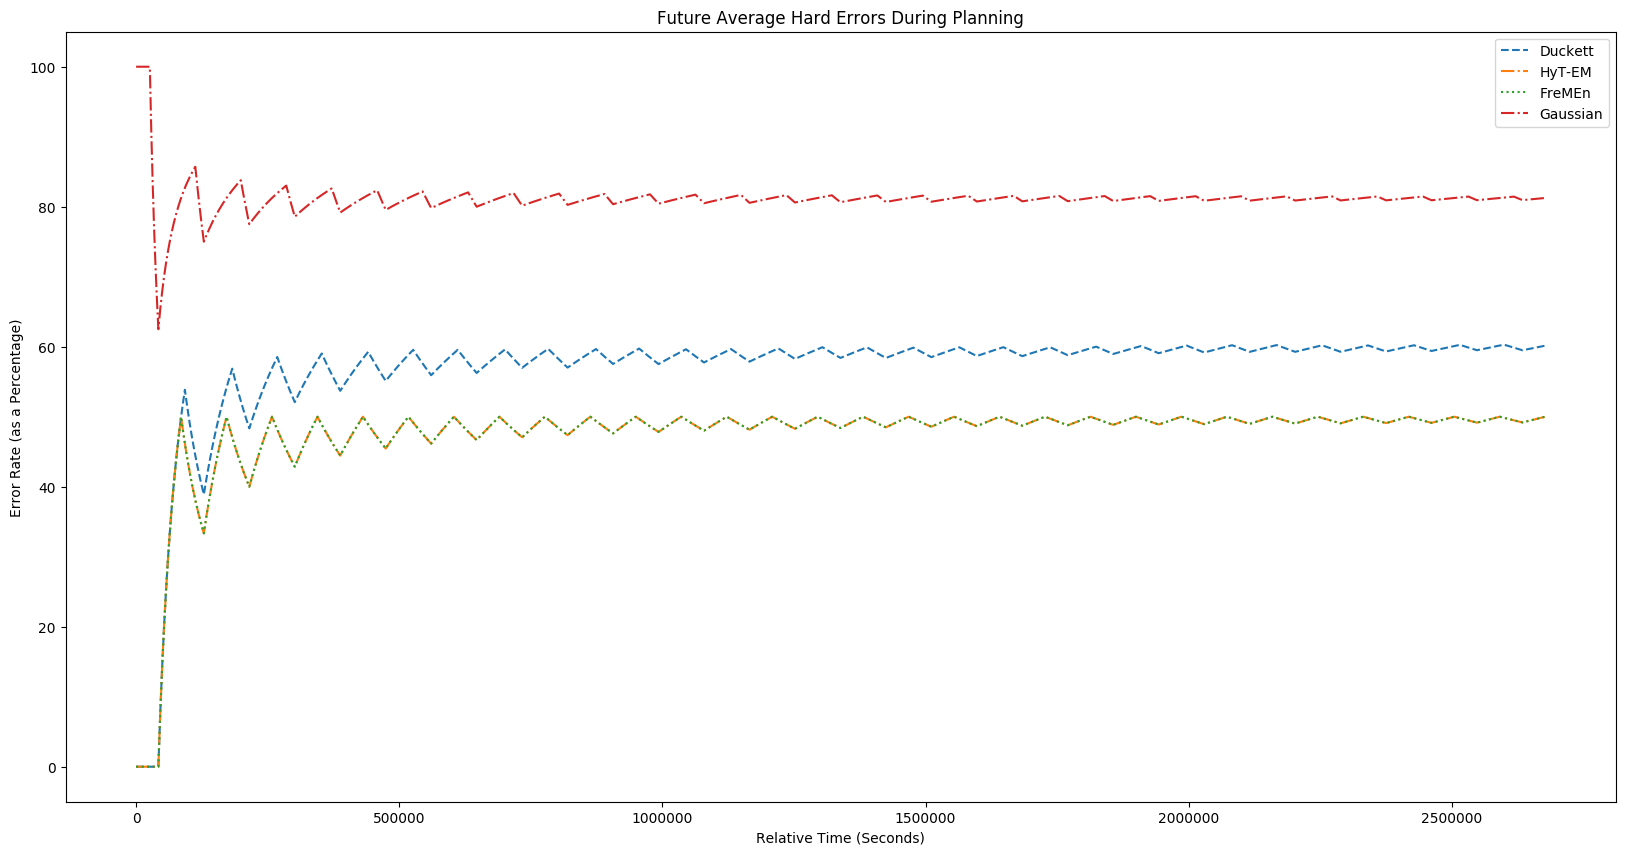
\includegraphics[width = 5in]{images/results/Future_Average_Hard_Errors_During_Planning.png}} \\
    {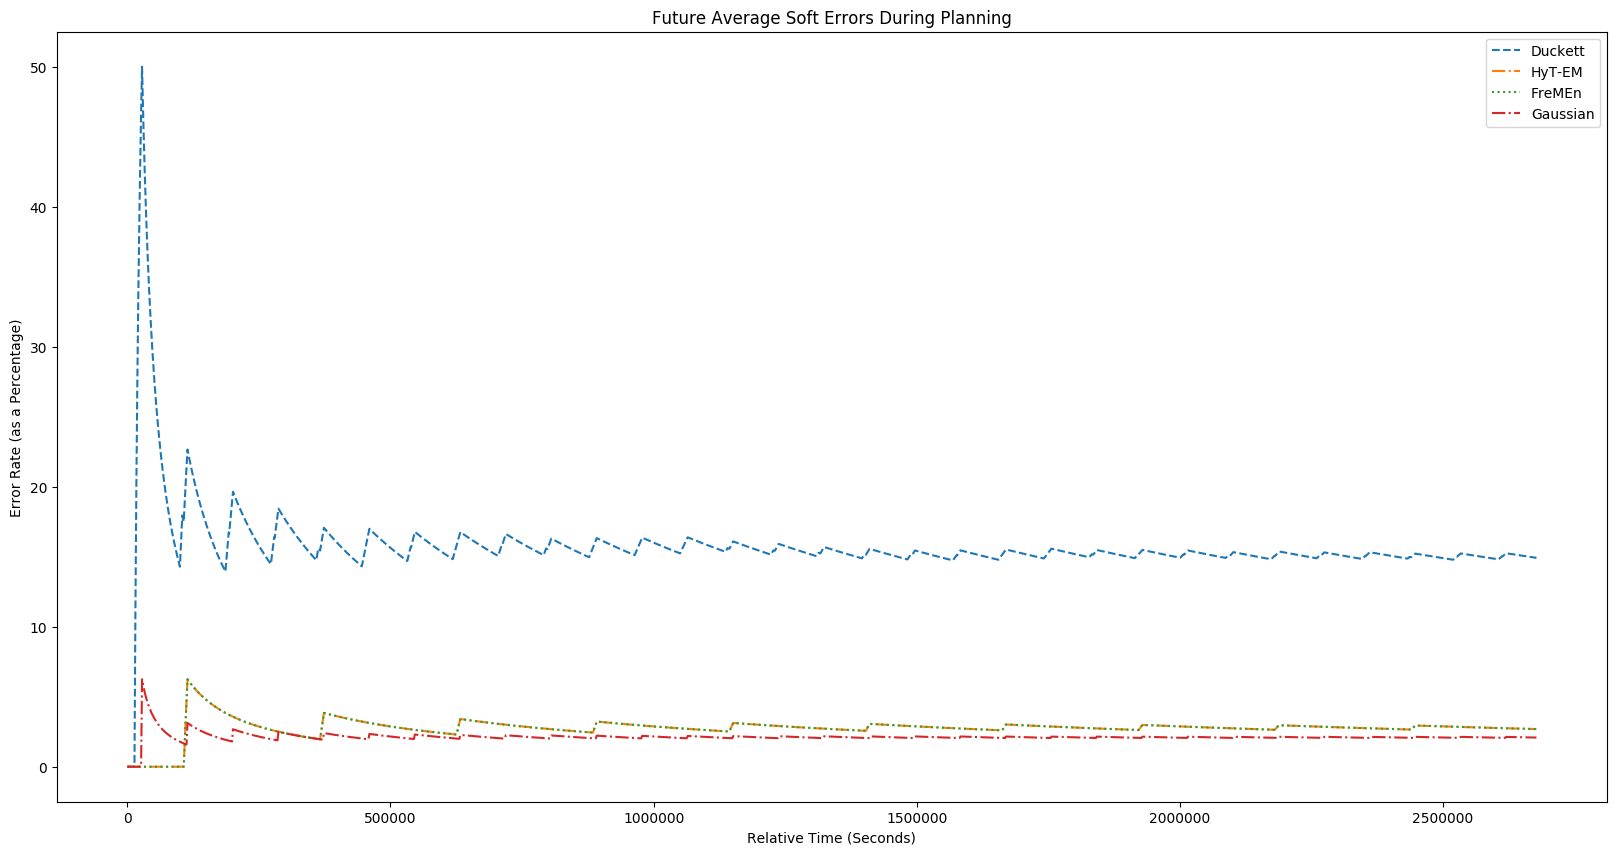
\includegraphics[width = 5in]{images/results/Future_Average_Soft_Errors_During_Planning.png}} \\
    {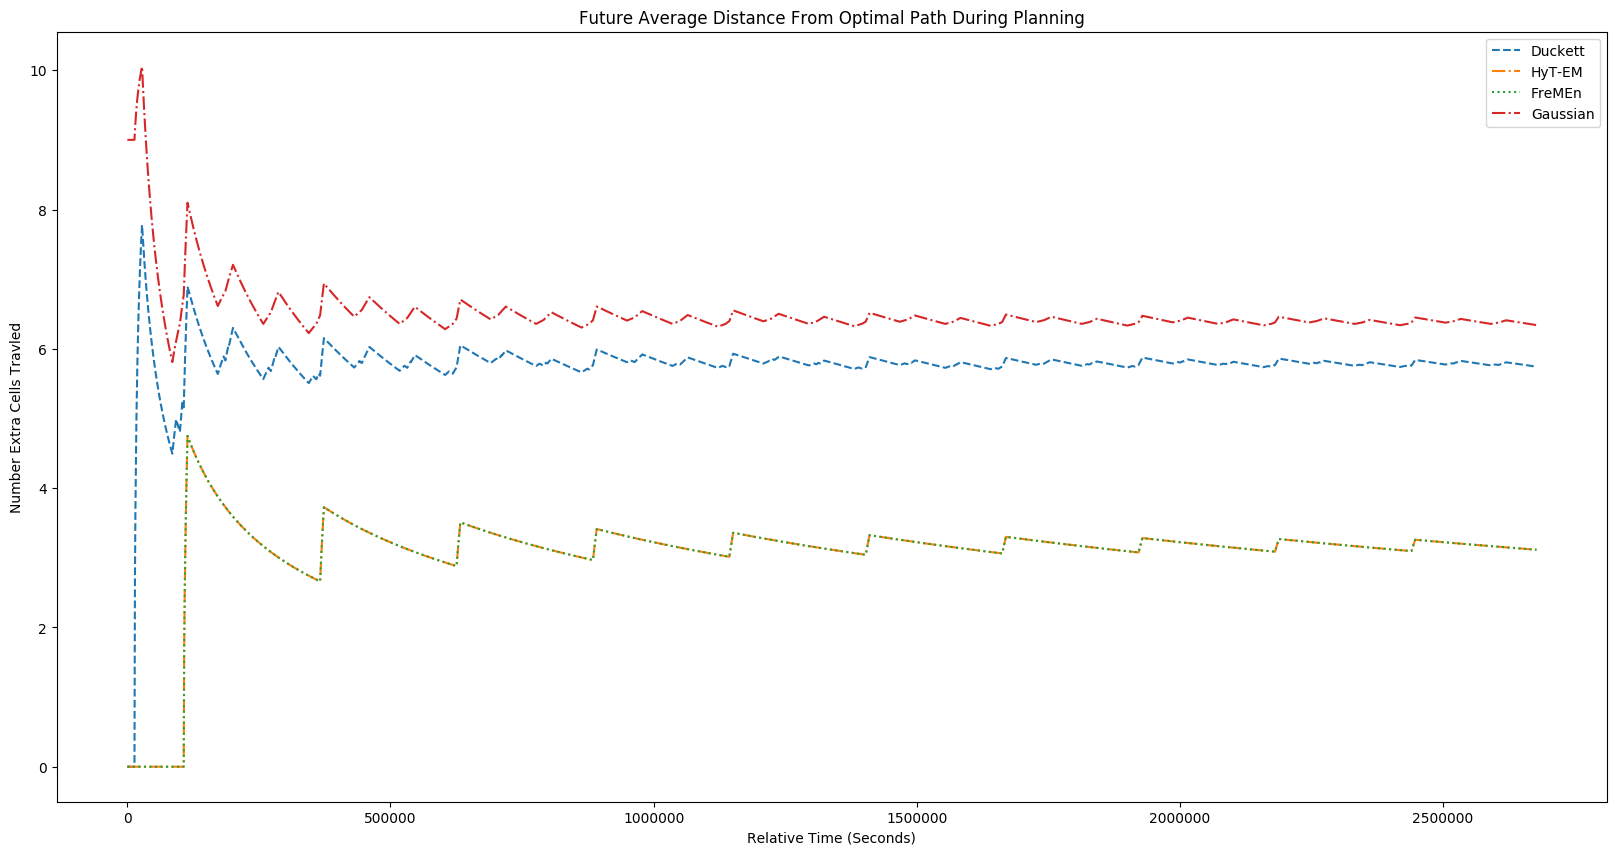
\includegraphics[width = 5in]{images/results/Future_Average_Distance_From_Optimal_Path_During_Planning.png}} \\
  \end{tabular}
  \caption{ Future Planning Results}
  \label{fig:G_FP_res}
\end{figure}







\begin{figure}
  \begin{tabular}{cc}
    {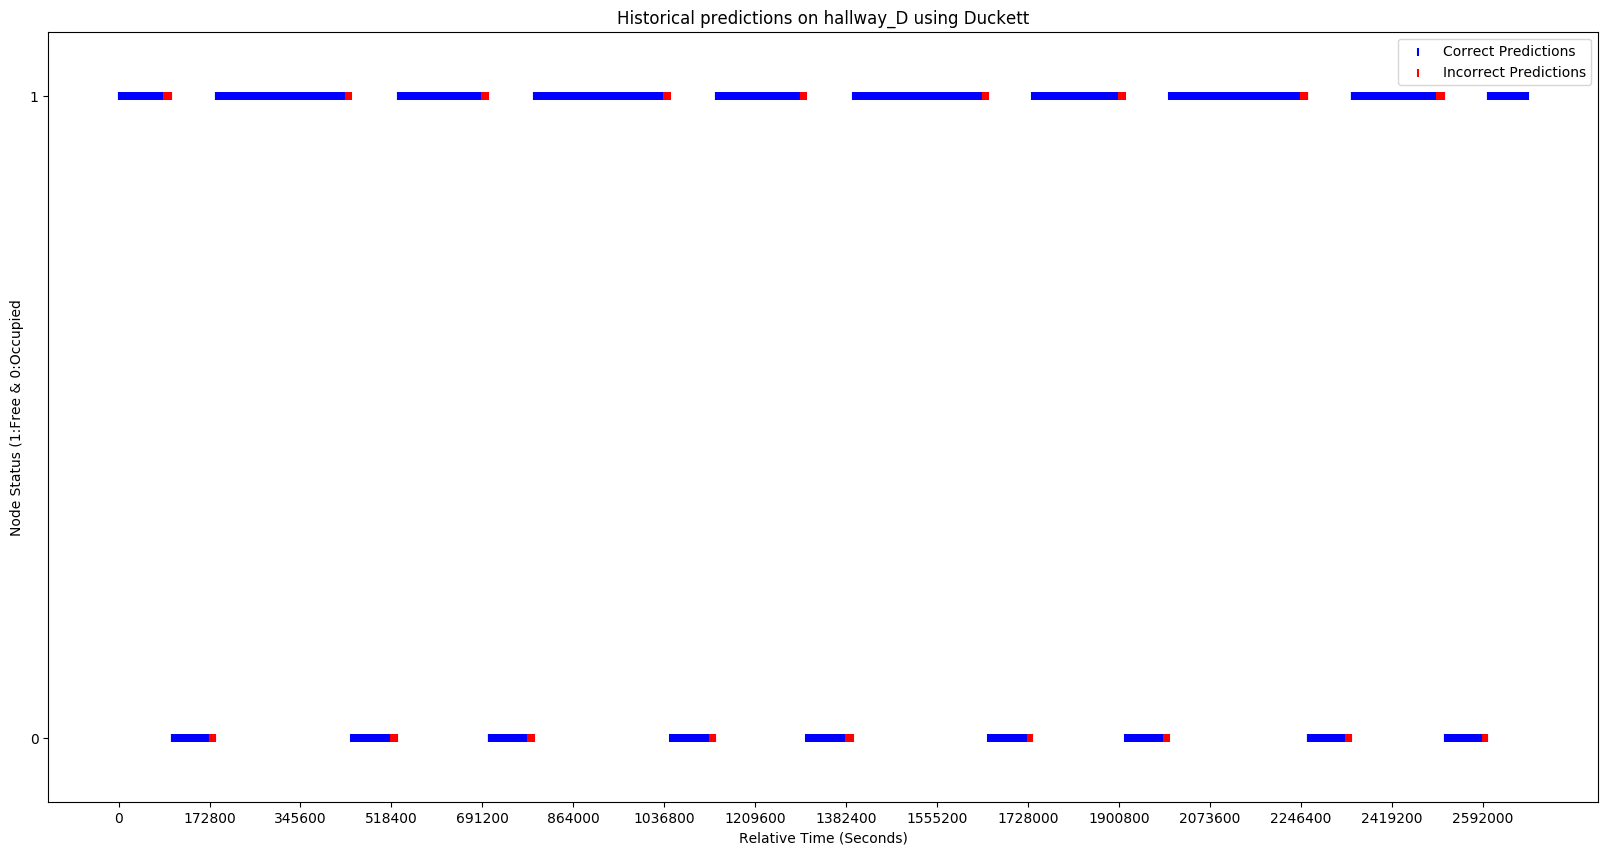
\includegraphics[width = 3in]{images/results/Historical_hallway_D_Duckett.png}} &
    {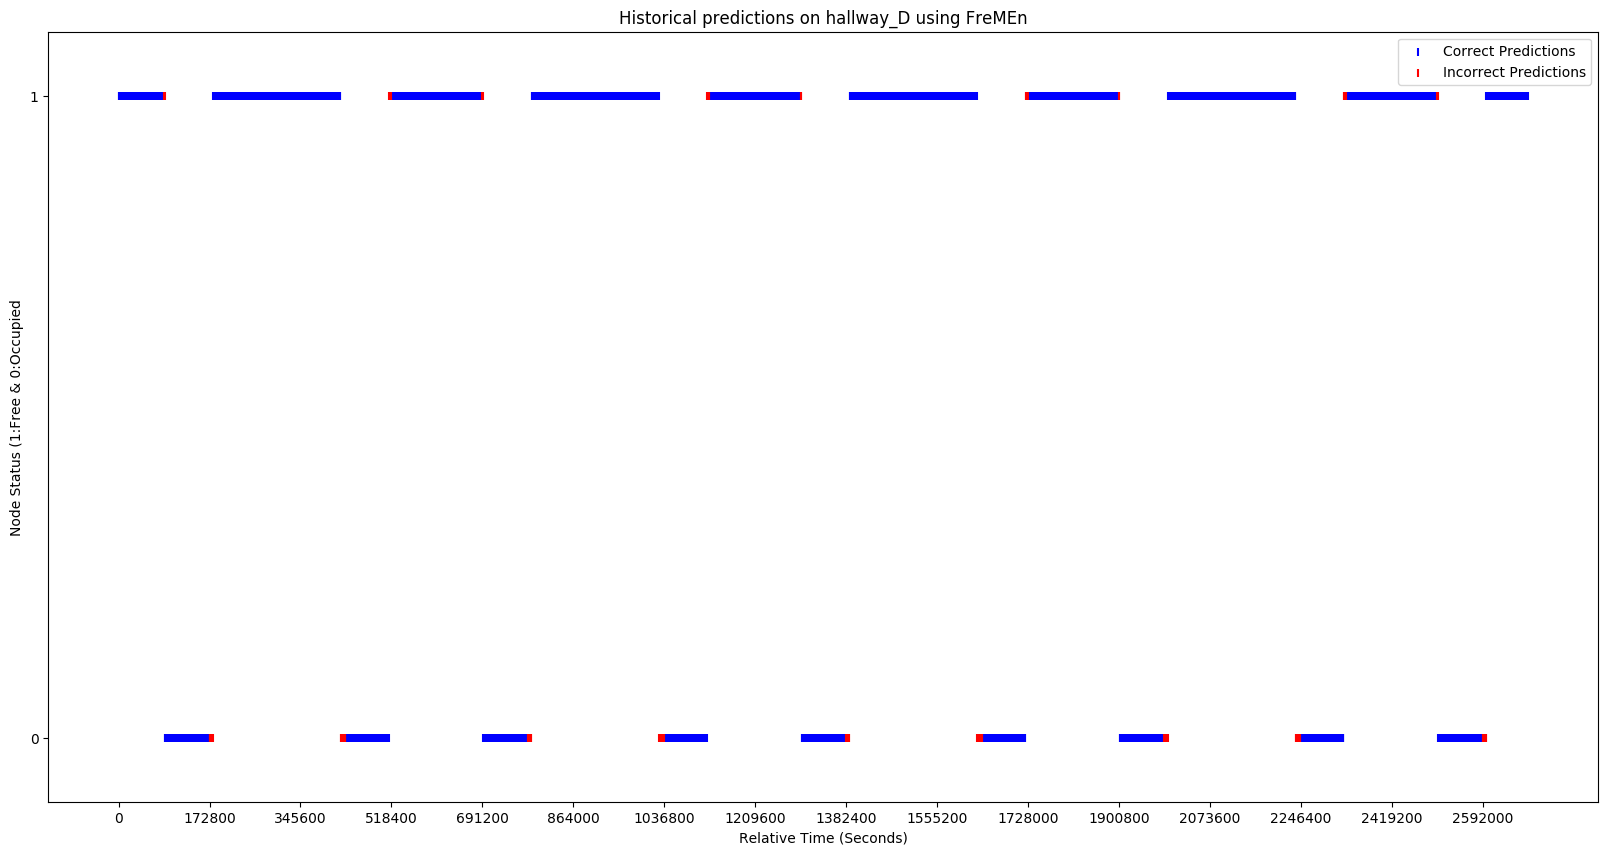
\includegraphics[width = 3in]{images/results/Historical_hallway_D_FreMEn.png}} \\
    {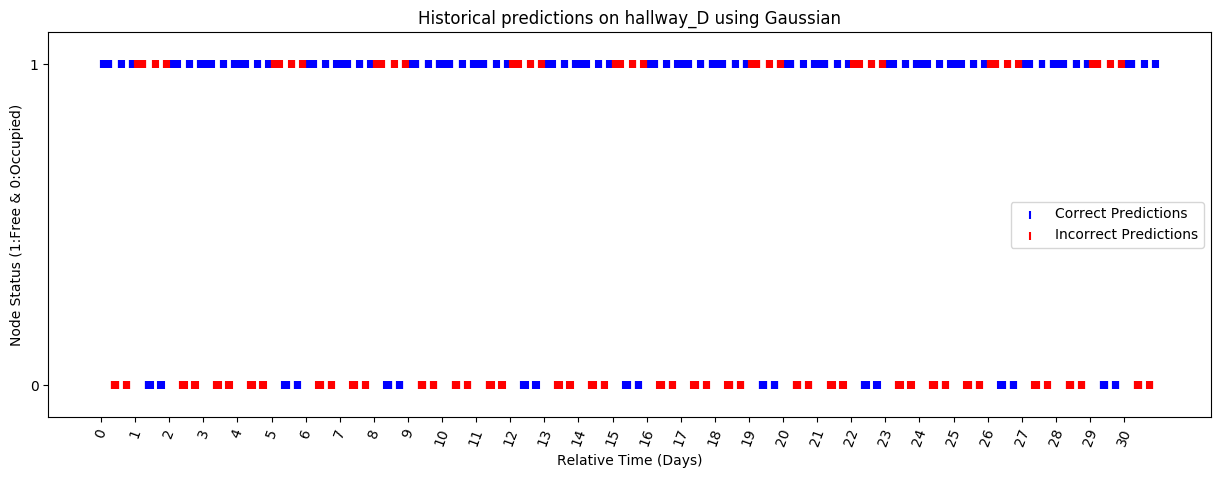
\includegraphics[width = 3in]{images/results/Historical_hallway_D_Gaussian.png}} &
    {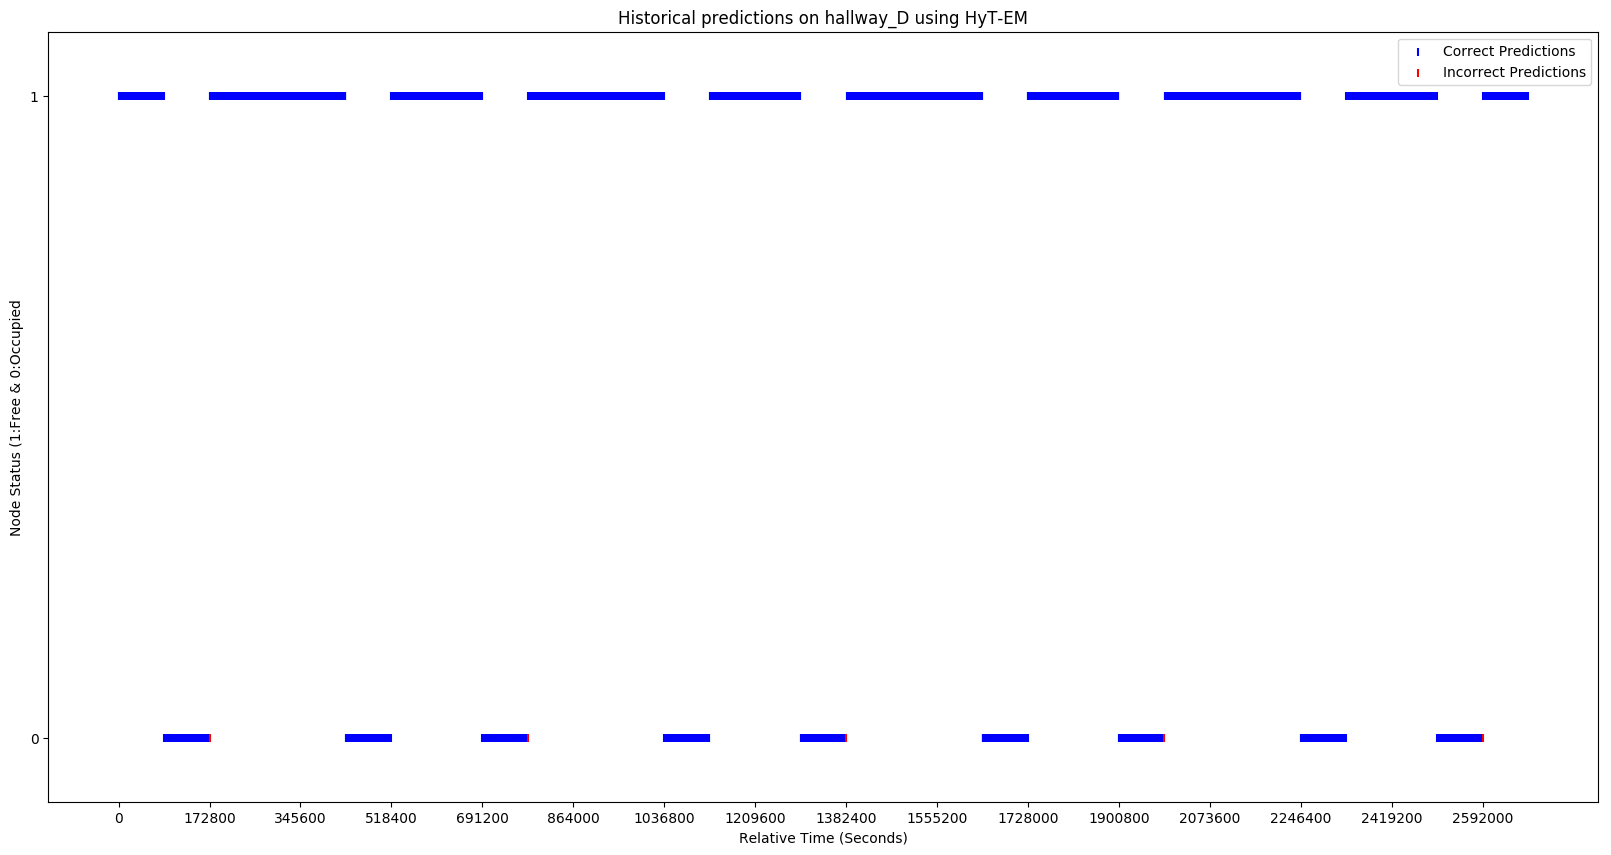
\includegraphics[width = 3in]{images/results/Historical_hallway_D_HyT-EM.png}} \\
  \end{tabular}
  \caption{Historical Recreations - Hallway Delivery}
\end{figure}\\ \\

\begin{figure}
  \begin{tabular}{cc}
    {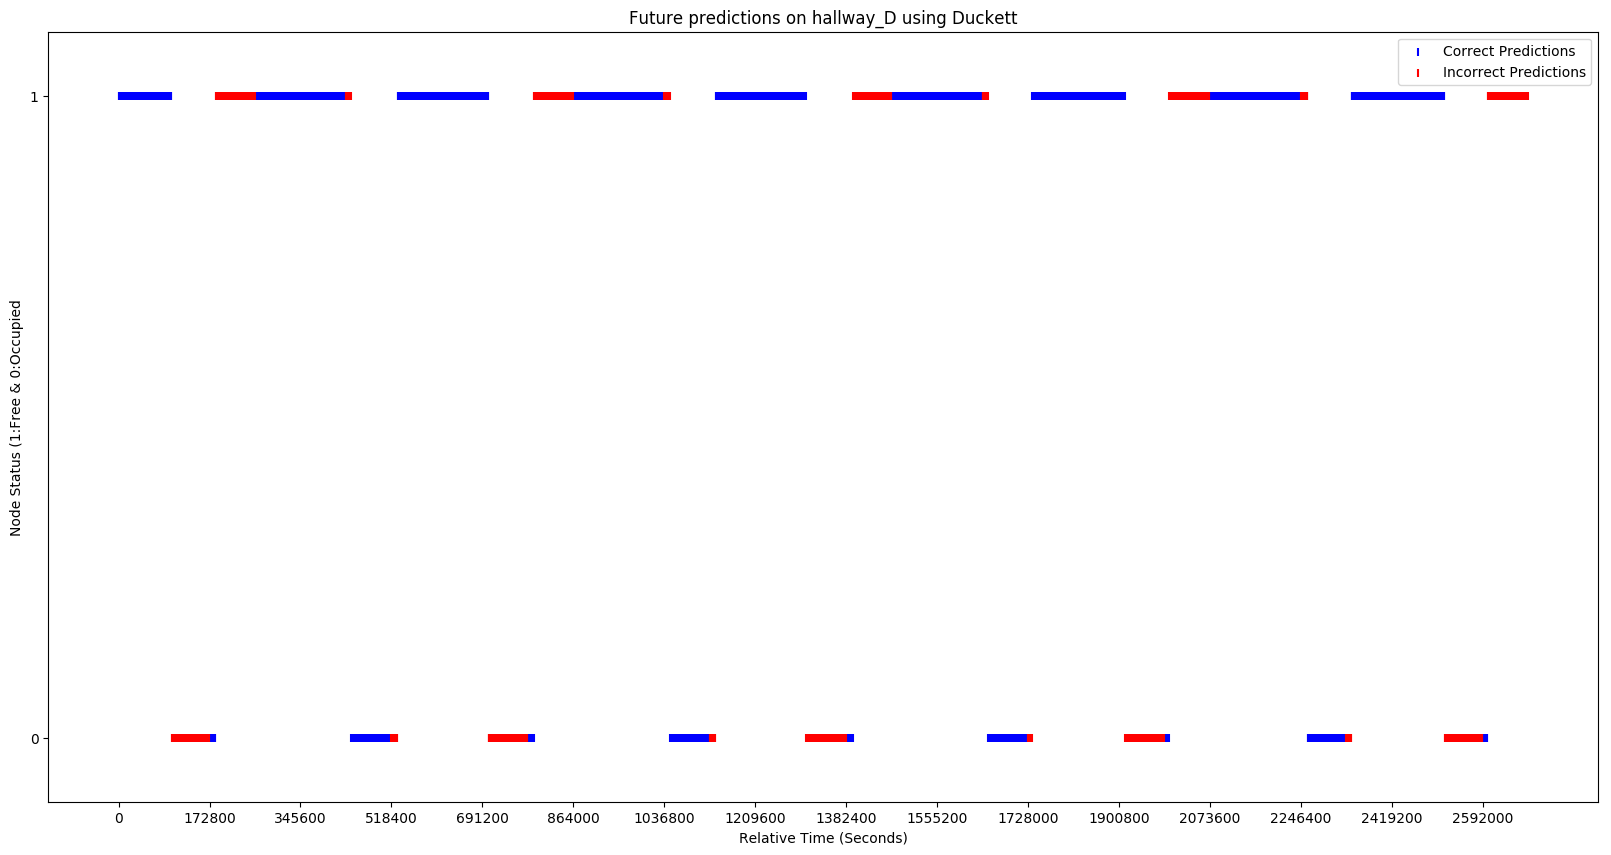
\includegraphics[width = 3in]{images/results/Future_hallway_D_Duckett.png}} &
    {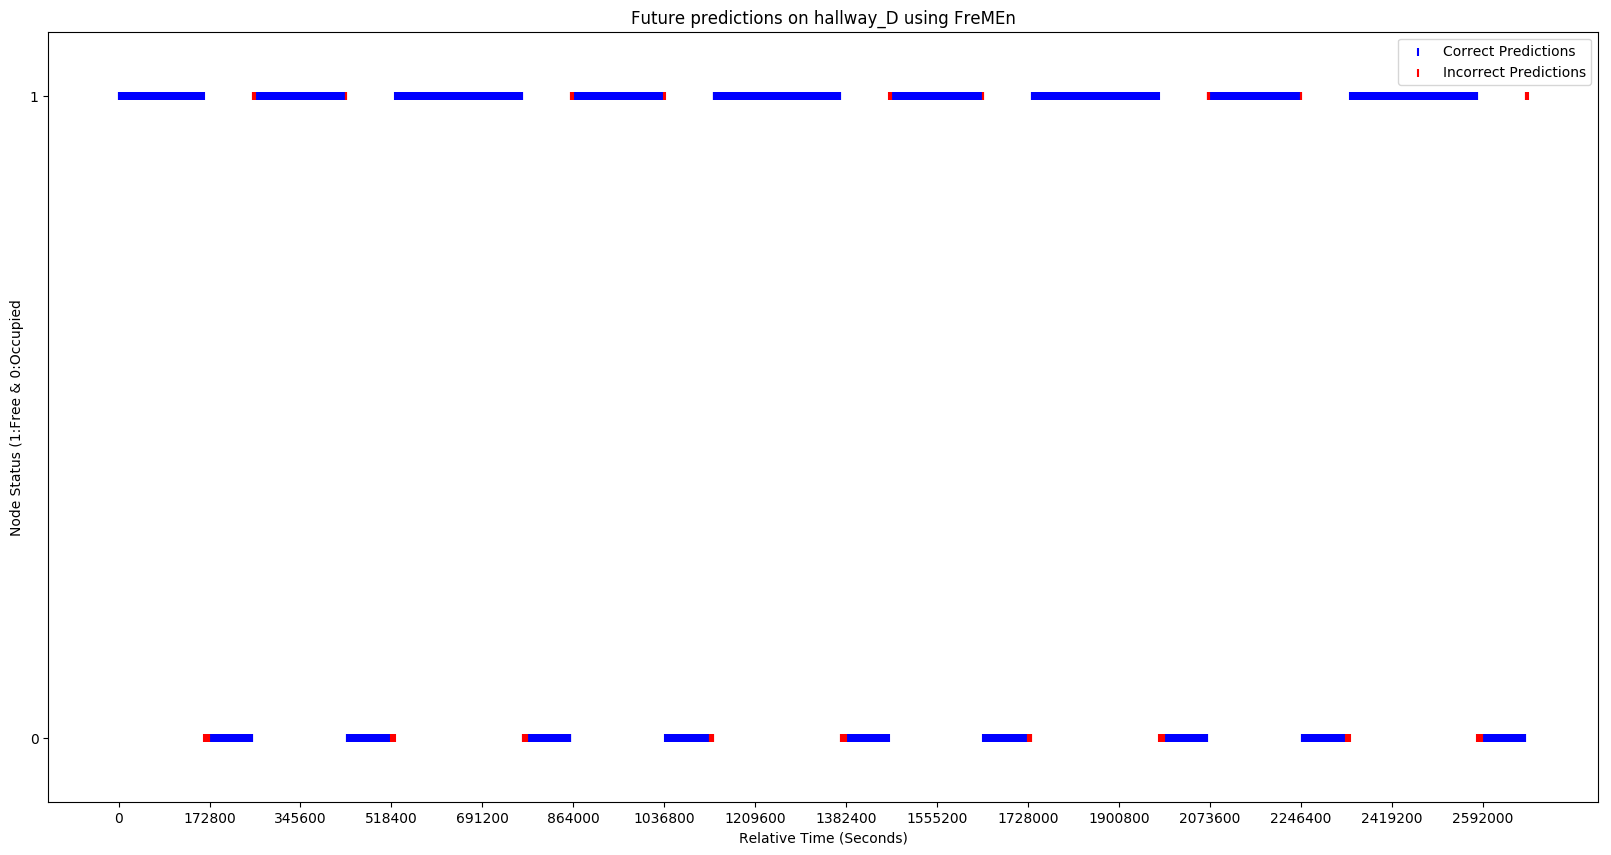
\includegraphics[width = 3in]{images/results/Future_hallway_D_FreMEn.png}} \\
    {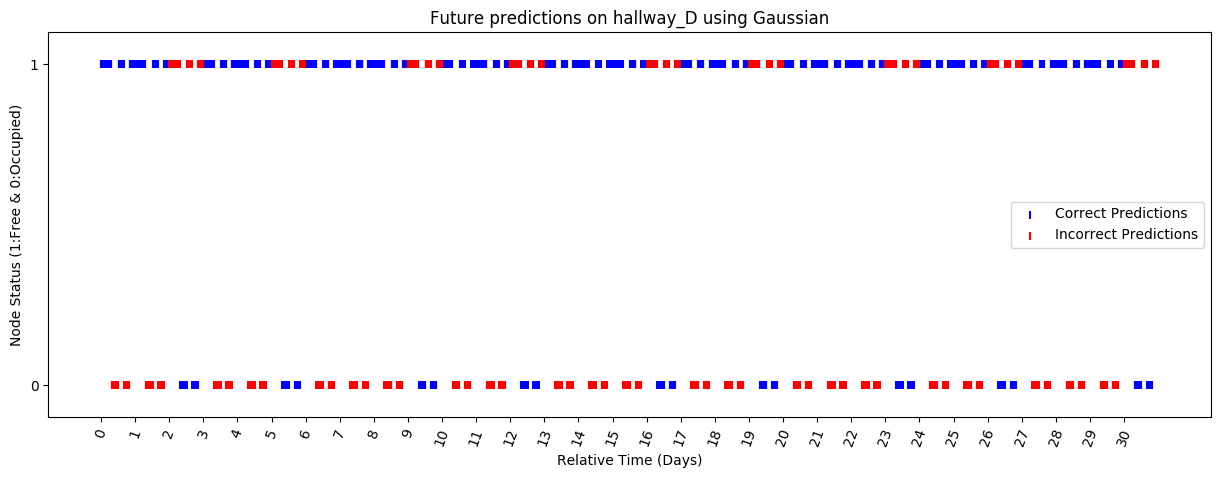
\includegraphics[width = 3in]{images/results/Future_hallway_D_Gaussian.png}} &
    {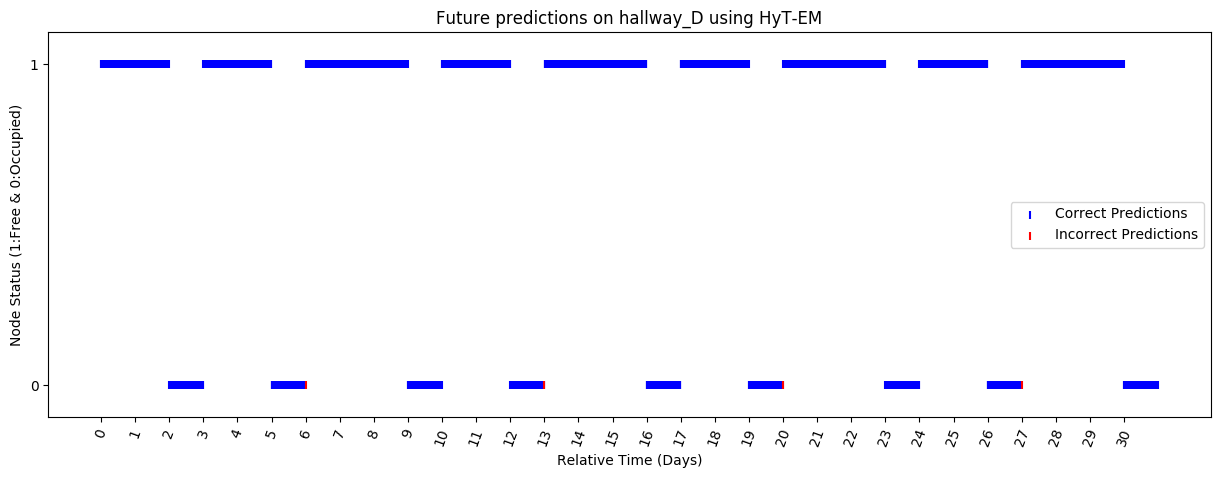
\includegraphics[width = 3in]{images/results/Future_hallway_D_HyT-EM.png}} \\
  \end{tabular}
  \caption{Future Predictions - Hallway Delivery}
\end{figure}\\ \\

\begin{figure}
  \begin{tabular}{cc}
    {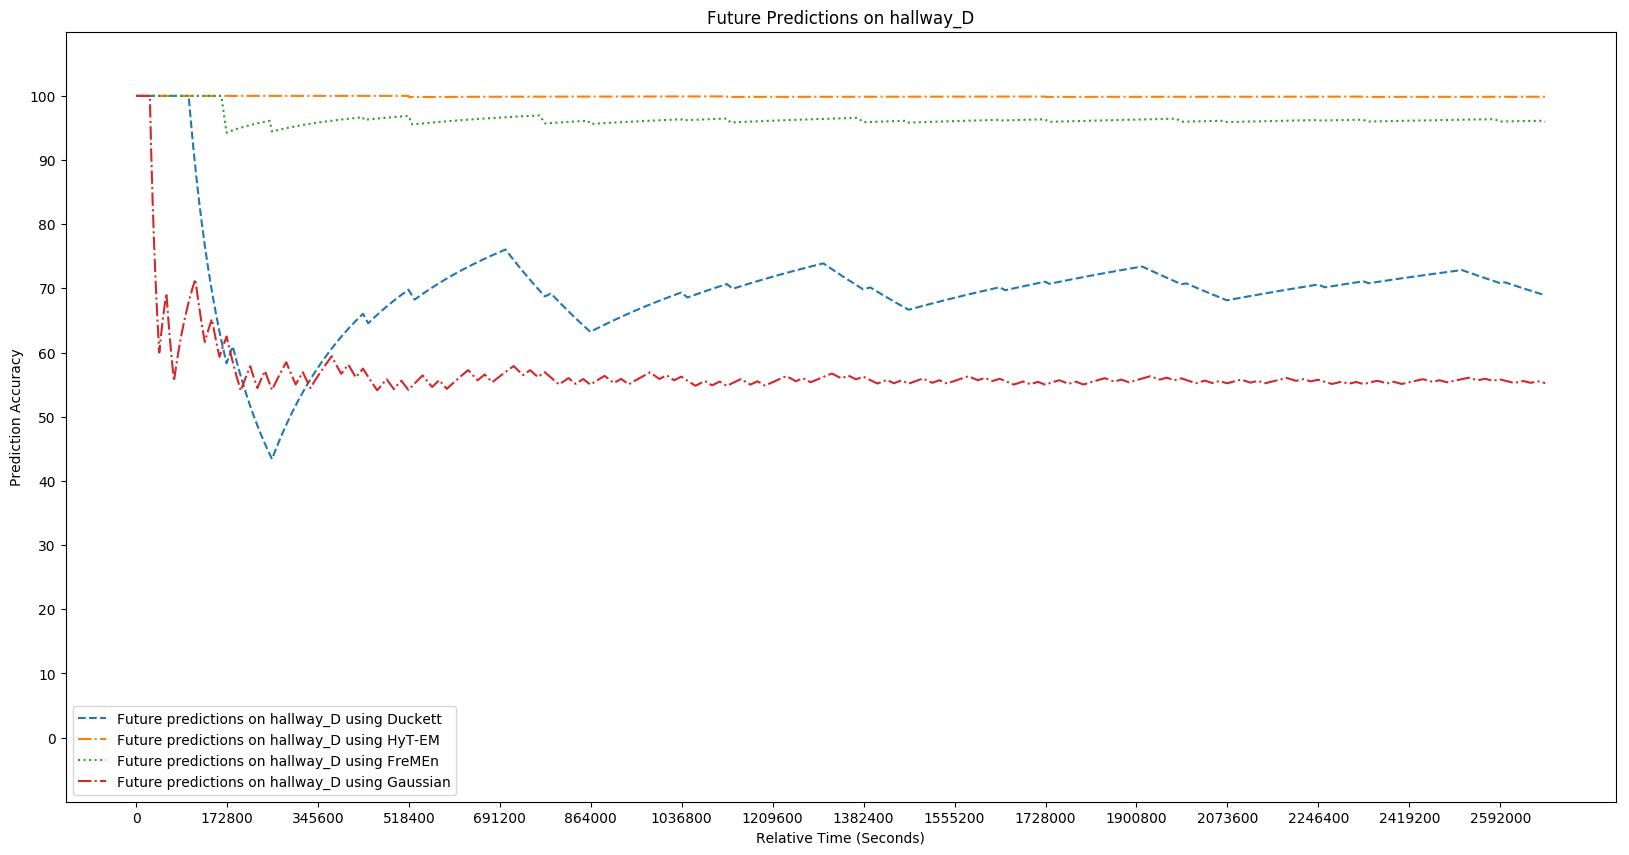
\includegraphics[width = 3in]{images/results/Future_Predictions_on_hallway_D.png}} &
    {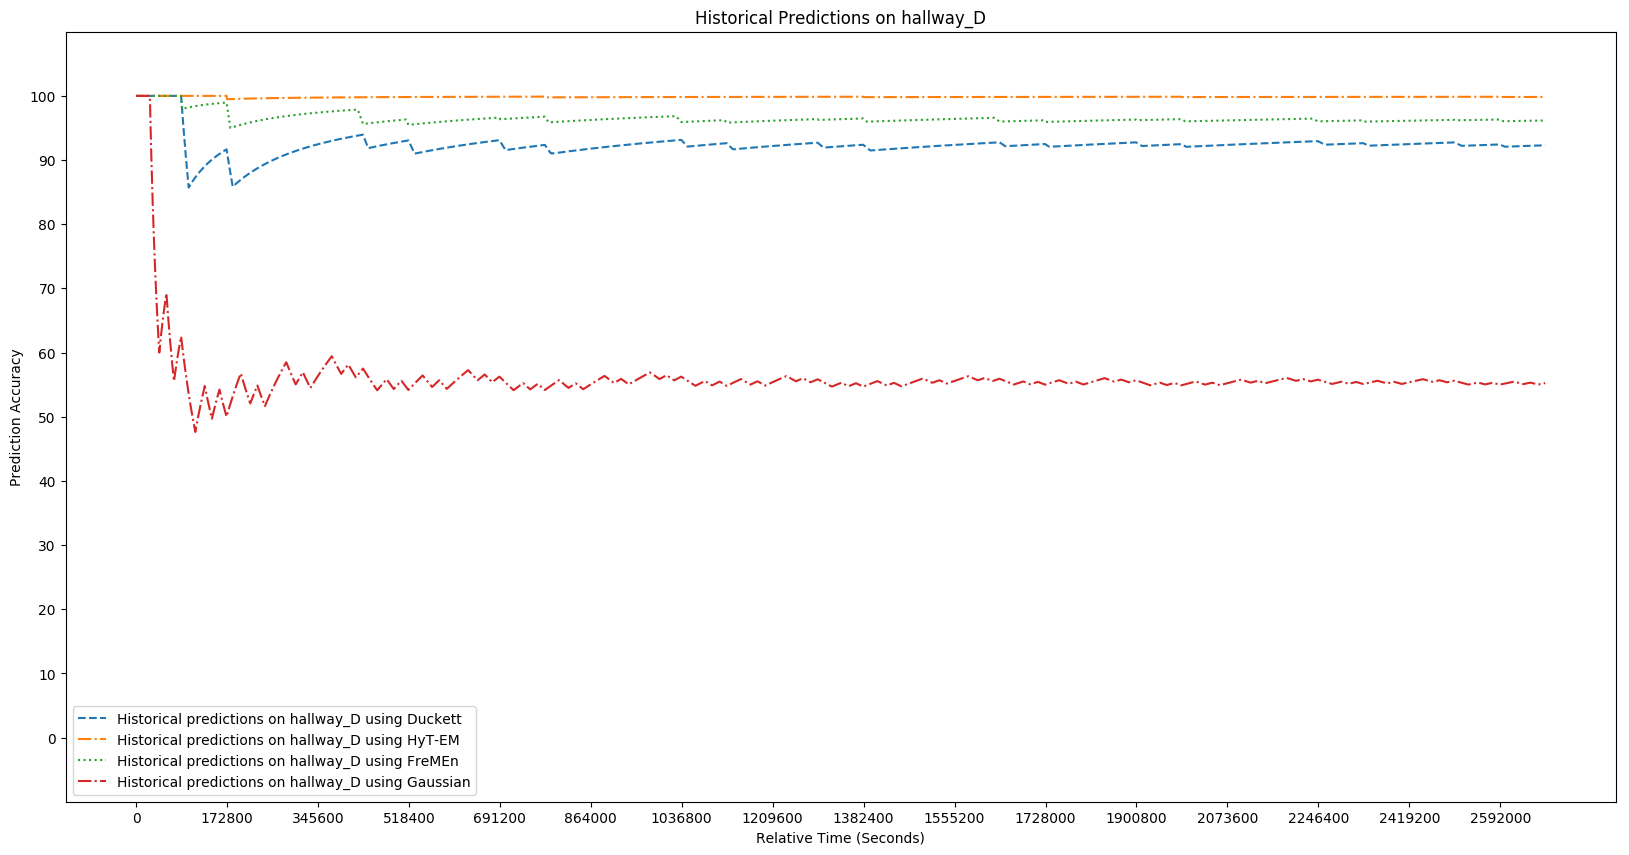
\includegraphics[width = 3in]{images/results/Historical_Predictions_on_hallway_D.png}} \\
  \end{tabular}
  \caption{Model Accuracy Over Time - Hallway Delivery}
\end{figure}\\ \\


\begin{figure}
  \begin{tabular}{cc}
    {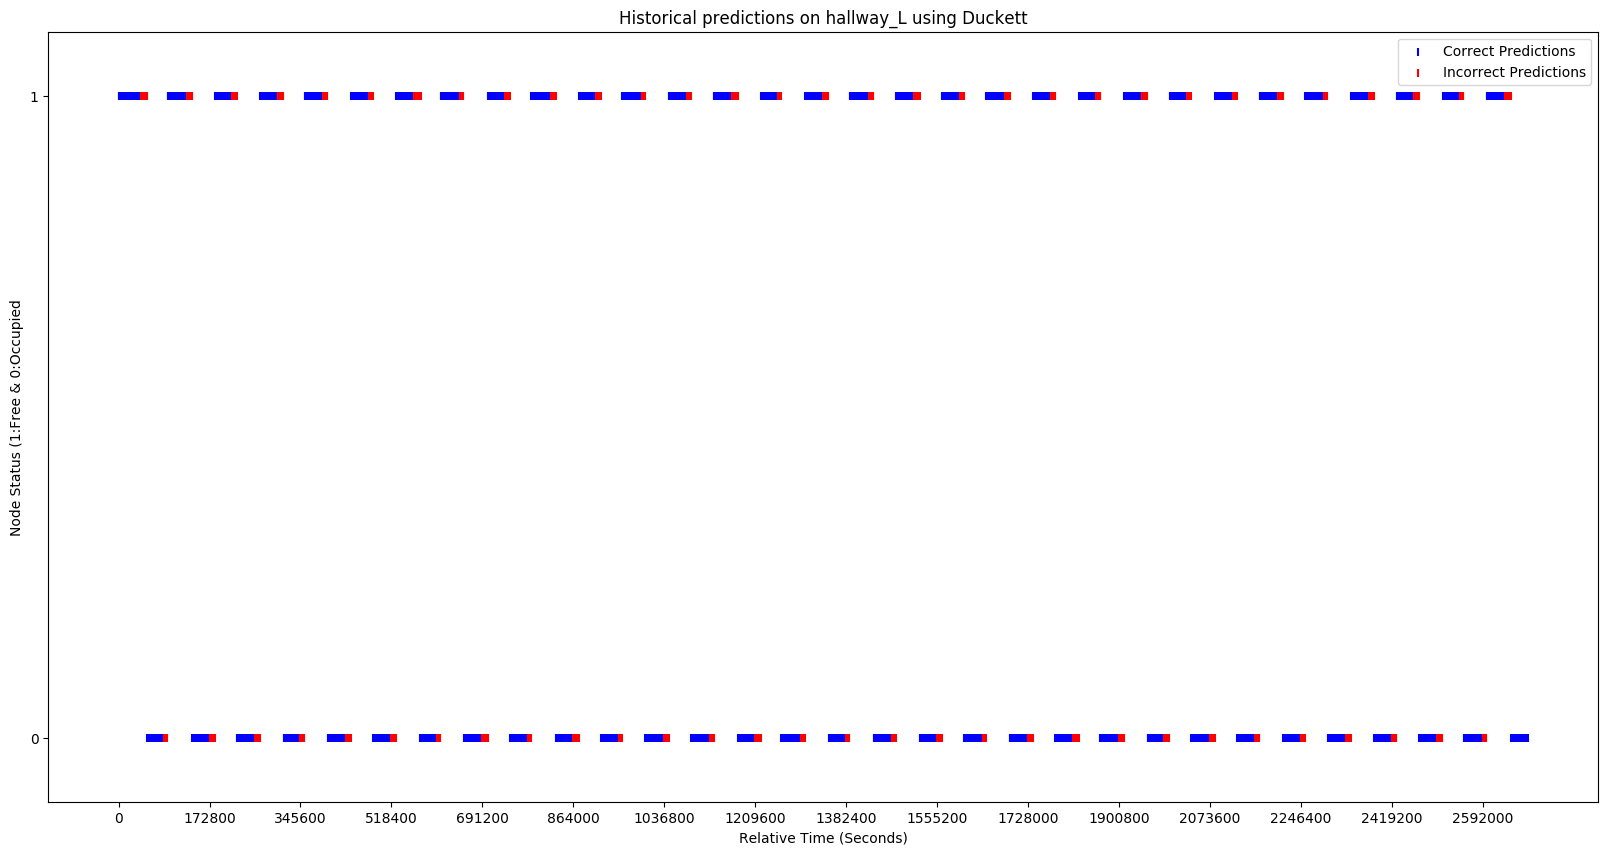
\includegraphics[width = 3in]{images/results/Historical_hallway_L_Duckett.png}} &
    {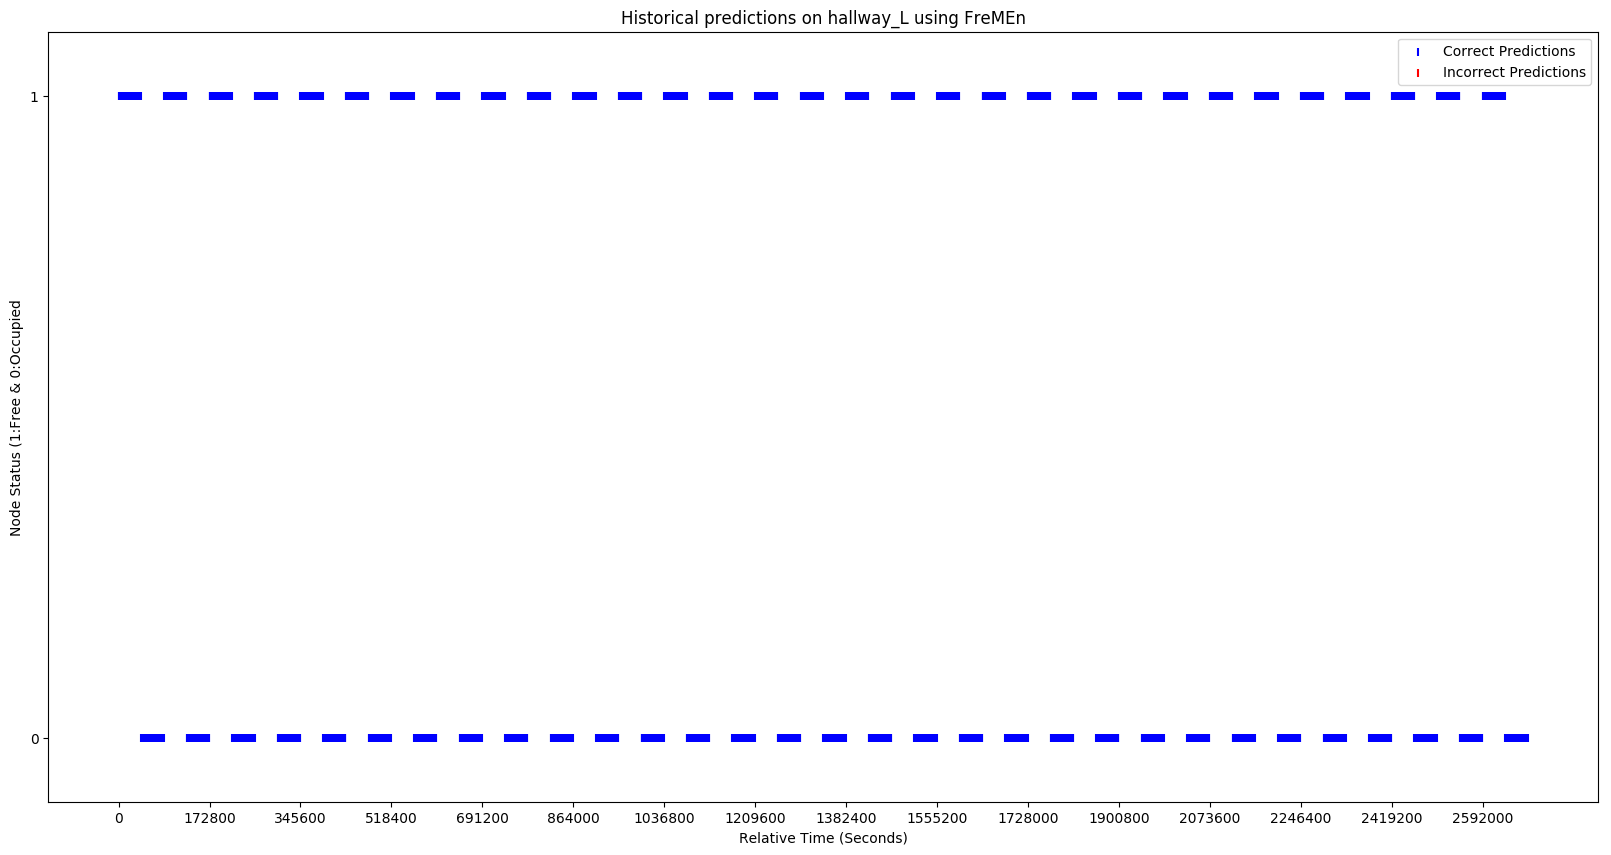
\includegraphics[width = 3in]{images/results/Historical_hallway_L_FreMEn.png}} \\
    {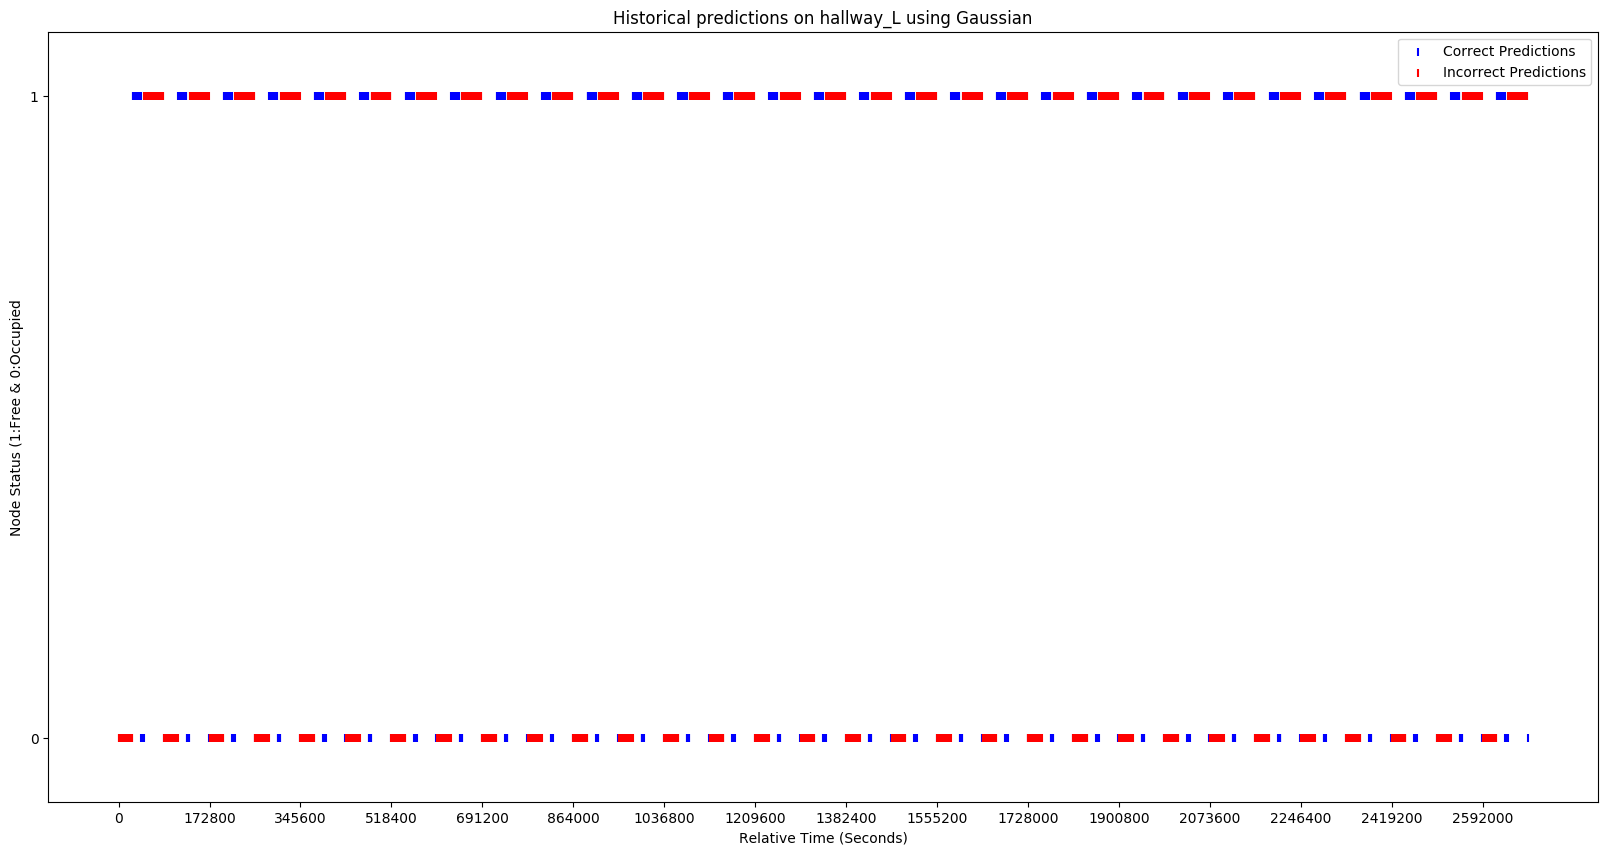
\includegraphics[width = 3in]{images/results/Historical_hallway_L_Gaussian.png}} &
    {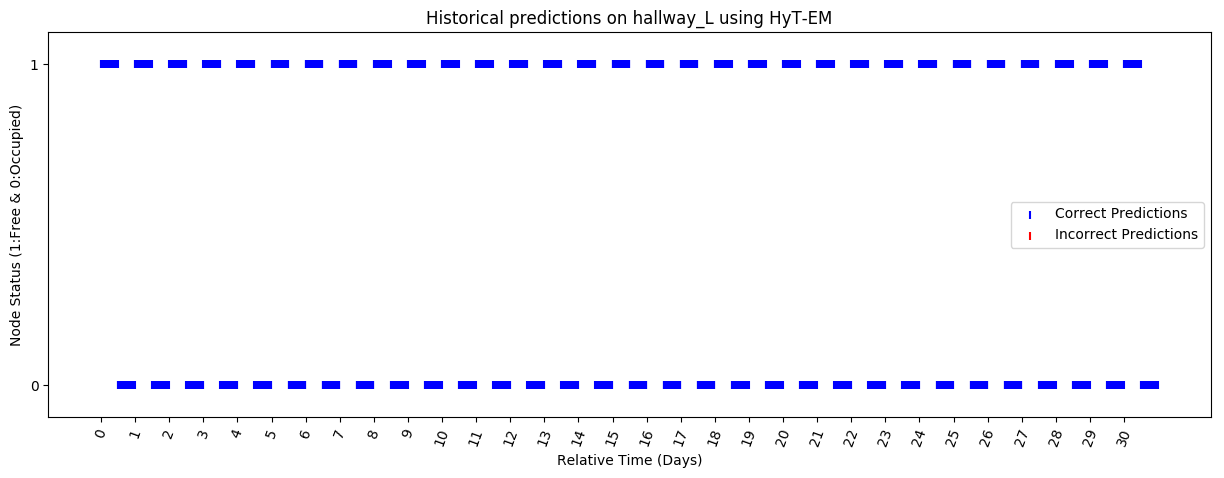
\includegraphics[width = 3in]{images/results/Historical_hallway_L_HyT-EM.png}} \\
  \end{tabular}
  \caption{Historical Recreations - Hallway Delivery}
\end{figure}

\begin{figure}
  \begin{tabular}{cc}
    {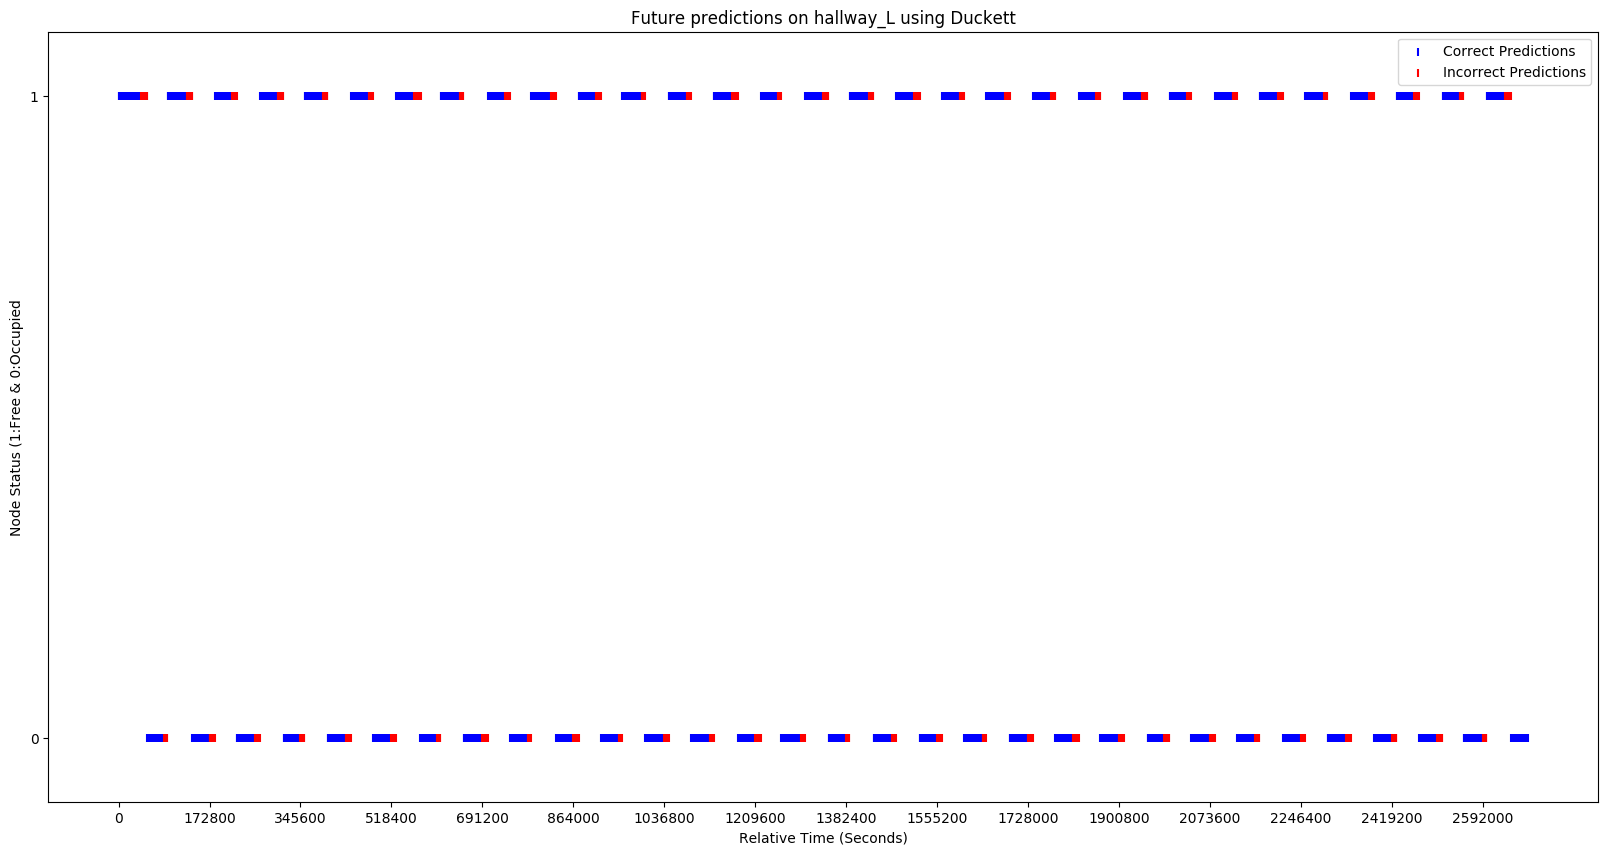
\includegraphics[width = 3in]{images/results/Future_hallway_L_Duckett.png}} &
    {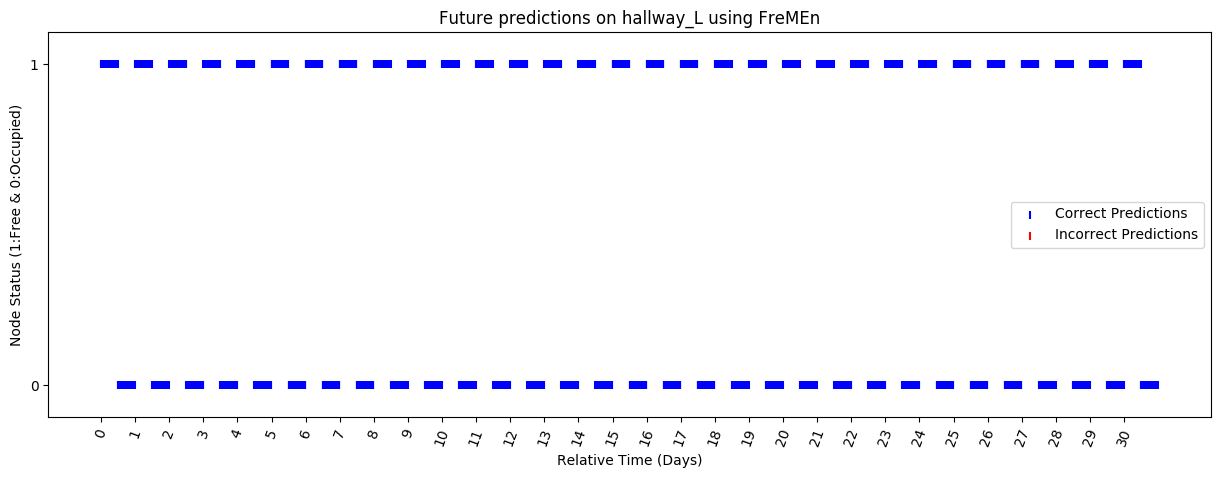
\includegraphics[width = 3in]{images/results/Future_hallway_L_FreMEn.png}} \\
    {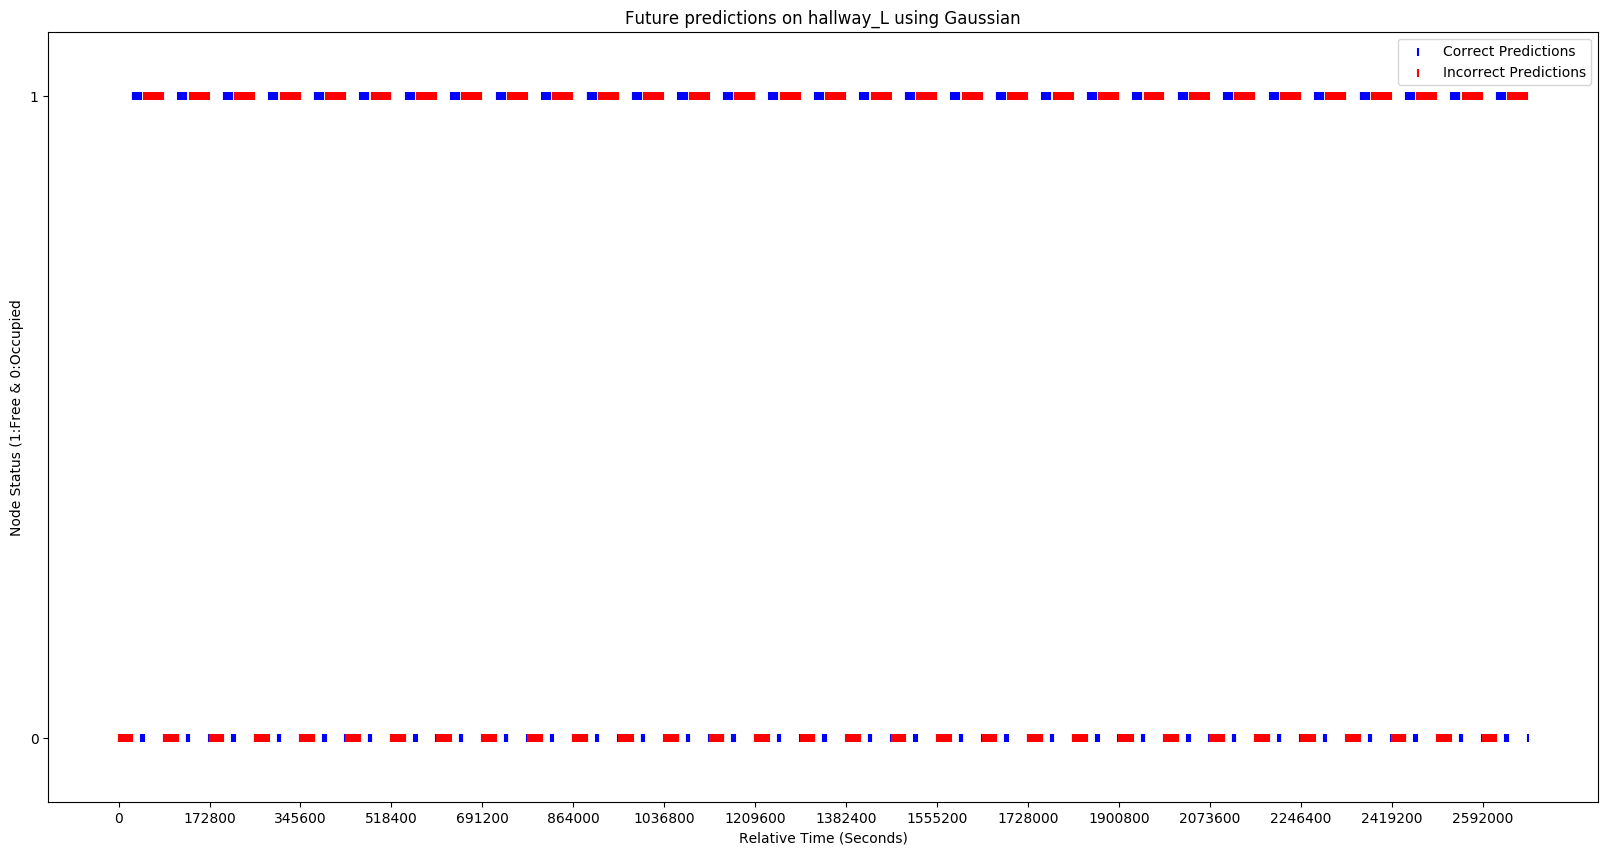
\includegraphics[width = 3in]{images/results/Future_hallway_L_Gaussian.png}} &
    {\includegraphics[width = 3in]{images/results/Future_hallway_L_HyT-EM.png}} \\
  \end{tabular}
  \caption{Future Predictions - Hallway Laundry}
\end{figure}

\begin{figure}
  \begin{tabular}{cc}
    {\includegraphics[width = 3in]{images/results/Future_Predictions_on_hallway_L.png}} &
    {\includegraphics[width = 3in]{images/results/Historical_Predictions_on_hallway_L.png}} \\
  \end{tabular}
  \caption{Model Accuracy Over Time - Hallway Laundry}
\end{figure}

\begin{figure}
  \begin{tabular}{cc}
    {\includegraphics[width = 3in]{images/results/Historical_hallway_M0_Duckett.png}} &
    {\includegraphics[width = 3in]{images/results/Historical_hallway_M0_FreMEn.png}} \\
    {\includegraphics[width = 3in]{images/results/Historical_hallway_M0_Gaussian.png}} &
    {\includegraphics[width = 3in]{images/results/Historical_hallway_M0_HyT-EM.png}} \\
  \end{tabular}
  \caption{Historical Recreations - Hallway Meal Section 0}
\end{figure}

\begin{figure}
  \begin{tabular}{cc}
    {\includegraphics[width = 3in]{images/results/Future_hallway_M0_Duckett.png}} &
    {\includegraphics[width = 3in]{images/results/Future_hallway_M0_FreMEn.png}} \\
    {\includegraphics[width = 3in]{images/results/Future_hallway_M0_Gaussian.png}} &
    {\includegraphics[width = 3in]{images/results/Future_hallway_M0_HyT-EM.png}} \\
  \end{tabular}
  \caption{Future Predictions - Hallway Meal Section 0}
\end{figure}

\begin{figure}
  \begin{tabular}{cc}
    {\includegraphics[width = 3in]{images/results/Future_Predictions_on_hallway_M0.png}} &
    {\includegraphics[width = 3in]{images/results/Historical_Predictions_on_hallway_M0.png}} \\
  \end{tabular}
  \caption{Model Accuracy Over Time - Hallway Meal Section 0}
\end{figure}



\begin{figure}
  \begin{tabular}{cc}
    {\includegraphics[width = 3in]{images/results/Historical_hallway_M1_Duckett.png}} &
    {\includegraphics[width = 3in]{images/results/Historical_hallway_M1_FreMEn.png}} \\
    {\includegraphics[width = 3in]{images/results/Historical_hallway_M1_Gaussian.png}} &
    {\includegraphics[width = 3in]{images/results/Historical_hallway_M1_HyT-EM.png}} \\
  \end{tabular}
  \caption{Historical Recreations - Hallway Meal Section 1}
\end{figure}

\begin{figure}
  \begin{tabular}{cc}
    {\includegraphics[width = 3in]{images/results/Future_hallway_M1_Duckett.png}} &
    {\includegraphics[width = 3in]{images/results/Future_hallway_M1_FreMEn.png}} \\
    {\includegraphics[width = 3in]{images/results/Future_hallway_M1_Gaussian.png}} &
    {\includegraphics[width = 3in]{images/results/Future_hallway_M1_HyT-EM.png}} \\
  \end{tabular}
  \caption{Future Predictions - Hallway Meal Section 1}
\end{figure}

\begin{figure}
  \begin{tabular}{cc}
    {\includegraphics[width = 3in]{images/results/Future_Predictions_on_hallway_M1.png}} &
    {\includegraphics[width = 3in]{images/results/Historical_Predictions_on_hallway_M1.png}} \\
  \end{tabular}
  \caption{Model Accuracy Over Time - Hallway Meal Section 1}
\end{figure}



\begin{figure}
  \begin{tabular}{cc}
    {\includegraphics[width = 3in]{images/results/Historical_hallway_T0_Duckett.png}} &
    {\includegraphics[width = 3in]{images/results/Historical_hallway_T0_FreMEn.png}} \\
    {\includegraphics[width = 3in]{images/results/Historical_hallway_T0_Gaussian.png}} &
    {\includegraphics[width = 3in]{images/results/Historical_hallway_T0_HyT-EM.png}} \\
  \end{tabular}
  \caption{Historical Recreations - Hallway Trash Section 0}
\end{figure}

\begin{figure}
  \begin{tabular}{cc}
    {\includegraphics[width = 3in]{images/results/Future_hallway_T0_Duckett.png}} &
    {\includegraphics[width = 3in]{images/results/Future_hallway_T0_FreMEn.png}} \\
    {\includegraphics[width = 3in]{images/results/Future_hallway_T0_Gaussian.png}} &
    {\includegraphics[width = 3in]{images/results/Future_hallway_T0_HyT-EM.png}} \\
  \end{tabular}
  \caption{Future Predictions - Hallway Trash Section 0}
\end{figure}

\begin{figure}
  \begin{tabular}{cc}
    {\includegraphics[width = 3in]{images/results/Future_Predictions_on_hallway_T0.png}} &
    {\includegraphics[width = 3in]{images/results/Historical_Predictions_on_hallway_T0.png}} \\
  \end{tabular}
  \caption{Model Accuracy Over Time - Hallway Trash Section 0}
\end{figure}



\begin{figure}
  \begin{tabular}{cc}
    {\includegraphics[width = 3in]{images/results/Historical_hallway_T1_Duckett.png}} &
    {\includegraphics[width = 3in]{images/results/Historical_hallway_T1_FreMEn.png}} \\
    {\includegraphics[width = 3in]{images/results/Historical_hallway_T1_Gaussian.png}} &
    {\includegraphics[width = 3in]{images/results/Historical_hallway_T1_HyT-EM.png}} \\
  \end{tabular}
  \caption{Historical Recreations - Hallway Trash Section 1}
\end{figure}

\begin{figure}
  \begin{tabular}{cc}
    {\includegraphics[width = 3in]{images/results/Future_hallway_T1_Duckett.png}} &
    {\includegraphics[width = 3in]{images/results/Future_hallway_T1_FreMEn.png}} \\
    {\includegraphics[width = 3in]{images/results/Future_hallway_T1_Gaussian.png}} &
    {\includegraphics[width = 3in]{images/results/Future_hallway_T1_HyT-EM.png}} \\
  \end{tabular}
  \caption{Future Predictions - Hallway Trash Section 1}
\end{figure}

\begin{figure}
  \begin{tabular}{cc}
    {\includegraphics[width = 3in]{images/results/Future_Predictions_on_hallway_T1.png}} &
    {\includegraphics[width = 3in]{images/results/Historical_Predictions_on_hallway_T1.png}} \\
  \end{tabular}
  \caption{Model Accuracy Over Time - Hallway Trash Section 1}
\end{figure}




\section{ Busy Elevators }

\subsection{ Classification Methods }

Upon even a cursory glance at the resulting graphs, such as the one in figure
~\ref{figure:Future_Recreations_-_Elevator_Data}, it is immediately
obvious that each model has a different approach to classification and
prediction of the data. Duckett, with the current prediction approach of
averaging each of its sub-models is perhaps the easiest to understand at first
glance. It results in a somewhat smooth curve that follows the training data
extremely closely. \\

Gaussian Mixture Models and FreMEn on the other hand, take a drastically
different approach.  Since, at their heart, they are binary classifiers, the
prediction methods as describe in Section 5 result into two distinct
prediction options. Both method's predictions hover around 0 and 7, although
not exactly on an integer boundary. It is clear the lower value is close to 0
due to the large amount of time the elevator spends at what is essentially a
rest state with next to no use. This is mostly between the hours of 22:00 and
08:30 or around 10 and a half hours. The other prediction that hovers around 7
is a bit harder to predict with precision but can roughly be estimated when
looking at the nominal times for waiting. When ruling out values that would be
placed into a 0 prediction we have a large amount of nominal values between 4
and 9 which averages out to 6.5. Finally, due to the large amount of noise
combined with the fact that an elevator cannot have a negative weight time,
the average is pulled up a bit by the extremely long wait times during rush
hours that can top 30 seconds.

Finally, and perhaps most interestingly, we have HyperTime. HyperTime takes an
interesting approach to classifying its data. Once again, looking at the figure
we can see that predictions are clustered on integer boundaries. To be clear,
non-binary HyperTime in its current implementation, although capable of training
on real data TODO foot note about real meaning float in CS it can only produce
integer predictions. This limitation is due to how predictions are evaluated
before being accepted as the actual prediction for a given time. TODO maybe
not source code but some pseudo code? When producing a prediction, or an
estimate as referred to in HyperTime, ``the likelihood distribution of the
sample having a given value at time t'' TODO site source code?! is calculated
for each sample from 0 until a maximum value. A maximum value for 30 was used
for this experiment. This means that HyperTime during calculation would never
be able to predict a wait time of 30 seconds or greater. Looking again at the
resulting figures, it is clear this is not an issue as there does not appear to
be any prediction greater than 10 seconds. Thus, with no predictions even
nearing 30, it is safe to say the upper limit did not hamper the ability for
the model to produce accurate predictions.

\subsection{ Metrics }

The only additional metric included in this experiment was that of ``Average
Distance from Correct Wait Time''. This, as the name implies, simply takes the
difference between a models predicted wait time and the ground truth wait time
provided in the data. The absolute value of this difference is saved and then
averaged for ever time step providing how the average changes over time. This
metric does not make a differentiation between the robot waiting for the
elevator versus the elevator waiting for the robot. No other additional
factors have been taken into account. This includes such things as calling an
elevator so far in advance that the elevator shows up and is called by someone
else

\subsection{ Performance \& Scalability }

\begin{table}[h!]
  \centering
  \resizebox{\textwidth}{!}{%
    \begin{tabular}{|l|l|l|l|l|}
      \hline
      & Duckett & Gaussian & FreMEn  & HyperTime \\ \hline
      Historical Average Additional Wait Time (Seconds)     & 3.05    & 3.24     & 2.13    & 1.90      \\ \hline
      Future Average Additional Wait Time (Seconds)         & 3.06    & 3.25     & 2.12    & 1.92      \\ \hline
      Computation Time (Milliseconds)                       & 610     & 60       & 70      & 7690      \\ \hline
      Memory Usage (KB)                                     & 31092   & 34636    & 34672   & 67788     \\ \hline
    \end{tabular}%
  }
  \caption{Elevator Wait Time Overview}
  \label{table:Elevator_Wait_Time_Overview}
\end{table}


\begin{table}[h!]
  \centering
  \resizebox{\textwidth}{!}{%
    \begin{tabular}{|l|l|l|l|l|}
      \hline
      & Duckett & Gaussian & FreMEn  & HyperTime \\ \hline
      Historical Average Additional Wait Time (Seconds)     & 1.58    & 4.47     & 2.05    & 1.58      \\ \hline
      Future Average Additional Wait Time (Seconds)         & 1.65    & 4.47     & 2.05    & 1.59      \\ \hline
      Computation Time (Milliseconds)                       & 7350    & 90       & 350     & 250037    \\ \hline
      Memory Usage (KB)                                     & 75304   & 35140    & 34980   & 79864     \\ \hline
    \end{tabular}%
  }
  \caption{High Resolution Elevator Wait Time Overview}
  \label{table:High_Resolution_Elevator_Wait_Time_Overview}
\end{table}

Table ~\ref{table:Elevator_Wait_Time_Overview} shows similar results to those
in previous sections with a few notable exceptions. To begin, computation time
remains mostly consistent with Gaussian Mixture Models and FreMEn coming in at
the upper tens of milliseconds with Duckett and order of magnitude higher and
HyperTime being yet another order of magnitude higher than Duckett. HyperTime
although still remaining under 10 seconds, does take slightly longer than would
be expected compared to previous results. This extra time is believed to originate
due to the switch from binary to non-binary classification. As mentioned previously,
when doing non-binary classification HyperTime must check every integer value
from 0 until a maximum prediction value, which in this case was 30. Had this
number been reduced to something closer to 10 (the maximum experimentally
predicted value) it is likely the computation time would have been reduced to
something closer to a two or three seconds placing it closer to previous
experiments but with a slightly longer time due to the additional calculations
needed. This same trend and affect is mirrored in memory usage for what is
assumed to be for the same reason. Finally, prediction wise, once again
similar results are visible. HyperTime has the best results with under 2
seconds of average distance from the correct wait time. Next comes FreMen
trailing just slightly behind at barely over 2 seconds. This is followed up
by Duckett and then Gaussian. \\

All said, the results are not too surprising when looking at previously ran
experiments, that is until the results in Table
~\ref{table:Elevator_Wait_Time_Overview} are compared with the results in Table
~\ref{table:High_Resolution_Elevator_Wait_Time_Overview}. The High Resolution
data, sampled at a rate of once per minute instead of once per 15 minutes really
exaggerates and exemplifies the data found in the lower resolution data. \\

Perhaps the most obvious and most interesting change is the drastic improvement
in Duckett. Duckett halved it's wait time error over the lower resolution data.
The main conclusion to be drawn from this is the importance of tuning Duckett
to refresh its internal representation of objects with the expected occurrence
of periodic changes with respect to the rate at which that data is being
sampled. Duckett struggles to predict changes in daily behavior when samples
occur at 15 minute increments as seen both in the low resolution data for the
elevator as well as the meal nodes back in the navigation experiment.
Additionally, a small decrease in wait time prediction is now much more obvious.
It is only a tenth of a second, so in the real-world this would not be too much
of an issue, but it again shows issues with long-term future predictions.

Slight movement is seen in either direction for Gaussian Mixture Models and
FreMEn. The simplistic nature of the Gaussian Mixture Models results in around
a second decrease in prediction accuracy but it does manage to maintain resource
usage very close to that of the lower density data. This suggest Gaussian
Mixture Models may be a good fit for very large datasets with simplistic
periodic behavior where precise accuracy is not necessary. FreMEn on the other
hand sees a slight increase in prediction accuracy but takes a bit of a hit
in computation time while maintaining memory usage. This additional hit in
computational time, specifically when compared to Gaussian Mixture Models,
is suspected to come from the model order FreMEn operates at (3) which causes
three loops through the training data for predictions. Since the loops are
merely over the same training data but with different parameters for estimation
it would make sense the computation time would increase but memory usage would
stay relatively similar. In fact, a rough calculation shows just this. Gaussian
Mixture Models take about 30 milliseconds longer in the high resolution data
an increase from 60 to 90. Adding an additional 30 milliseconds to FreMEn's
low resolution computation time value of 70 gives up 100 milliseconds. Accounting
for the additional work done by FreMEn by multiplying by 3 yields around 300
milliseconds. This is close to the observed 350 milliseconds especially when
additional overhead is considered. \\

Finally, HyperTime has arguably the most intriguing change between high and low
resolution elevator data. There is a relatively small increase in memory usage
but nothing out of the ordinary. The computational usage, however, sees an
extremely large increase to over 250000 milliseconds or over 4 minutes. This
additional run time only yields a performance increase of between 300 and 400
milliseconds. It may be argued that the relatively small increase of prediction
accuracy may be due to HyperTime running into an inability to make more accurate
predictions due to its integer limitation. Without this limitation it could
perhaps continue to increase in accuracy but this would only further harm its
computational time. The computational time is predicted to have scaled so poorly
due to the large number of calculations done for each data point during the
estimation portion of prediction. As noted previously, in this specific case
30 complex calculations must be done for a single estimation can be chosen at
a given time t. It is important to note that a reduction in the maximum
prediction value, as mentioned previously, would most likely reduce the
computational time considerably. Perhaps as much as a third of it's original
value if the max estimate was limited to 10. This would result in a
computational time closer to a minute to a minute and a half to 2 minute and a
half to 2 minutes.




\begin{figure}
  \begin{tabular}{cc}
    {\includegraphics[width = 3in]{images/results/Historical_elevator_Duckett.png}} &
    {\includegraphics[width = 3in]{images/results/Historical_elevator_FreMEn.png}} \\
    {\includegraphics[width = 3in]{images/results/Historical_elevator_Gaussian.png}} &
    {\includegraphics[width = 3in]{images/results/Historical_elevator_HyT-EM.png}} \\
  \end{tabular}
  \caption{Historical Recreations - Elevator Data}
  \label{figure:Historical_Recreations_-_Elevator_Data}
\end{figure}

\begin{figure}
  \begin{tabular}{cc}
    {\includegraphics[width = 3in]{images/results/Future_elevator_Duckett.png}} &
    {\includegraphics[width = 3in]{images/results/Future_elevator_FreMEn.png}} \\
    {\includegraphics[width = 3in]{images/results/Future_elevator_Gaussian.png}} &
    {\includegraphics[width = 3in]{images/results/Future_elevator_HyT-EM.png}} \\
  \end{tabular}
  \caption{Future Predictions - Elevator Data}
  \label{figure:Future_Predictions_-_Elevator_Data}
\end{figure}

\begin{figure}
  \begin{tabular}{cc}
    {\includegraphics[width = 3in]{images/results/Future_Predictions_on_Elevator_Data.png}} &
    {\includegraphics[width = 3in]{images/results/Historical_Predictions_on_Elevator_Data.png}} \\
  \end{tabular}
  \caption{Model Accuracy Over Time - Elevator Data}
  \label{figure:Model_Accuracy_Over_Time_-_Elevator_Data}
\end{figure}

\begin{figure}
  \begin{tabular}{cc}
    {\includegraphics[width = 3in]{images/results/Historical_high_res_elevator_Duckett.png}} &
    {\includegraphics[width = 3in]{images/results/Historical_high_res_elevator_FreMEn.png}} \\
    {\includegraphics[width = 3in]{images/results/Historical_high_res_elevator_Gaussian.png}} &
    {\includegraphics[width = 3in]{images/results/Historical_high_res_elevator_HyT-EM.png}} \\
  \end{tabular}
  \caption{Historical Recreations - High Resolution Elevator Data}
  \label{figure:Historical_Recreations_-_High_Resolution_Elevator_Data}
\end{figure}

\begin{figure}
  \begin{tabular}{cc}
    {\includegraphics[width = 3in]{images/results/Future_high_res_elevator_Duckett.png}} &
    {\includegraphics[width = 3in]{images/results/Future_high_res_elevator_FreMEn.png}} \\
    {\includegraphics[width = 3in]{images/results/Future_high_res_elevator_Gaussian.png}} &
    {\includegraphics[width = 3in]{images/results/Future_high_res_elevator_HyT-EM.png}} \\
  \end{tabular}
  \caption{Future Predictions - High Resolution Elevator Data}
  \label{figure:Future_Predictions_-_High_Resolution_Elevator_Data}
\end{figure}

\begin{figure}
  \begin{tabular}{cc}
    {\includegraphics[width = 3in]{images/results/Future_Predictions_on_Elevator_Data_High_Res.png}} &
    {\includegraphics[width = 3in]{images/results/Historical_Predictions_on_Elevator_Data_High_Res.png}} \\
  \end{tabular}
  \caption{Model Accuracy Over Time - High Resolution Elevator Data}
  \label{figure:Model_Accuracy_Over_Time_-_High_Resolution_Elevator_Data}
\end{figure}


\subsection{ Final Thoughts }
In terms of memory usage, all four methods appear to be relatively similar, which is to be expected.
Duckett good at
Fourier good at

\end{document}
